\section{Principles of photoacoustics}

For a basic understanding, this section will give a short introduction into the underlying photoacoustic effect and continues with its applications to microscopy. Furthermore, the used setup for the measurements gets discussed.

\subsection{Photoacoustic effect}
\label{sec:photoeffect}
The generation of a photoacoustic wave due to the illumination of a sample with temporal modulated light follows the process shown in Figure \ref{fig:PAgen} \cite{Wang:PAMtutorial}. 

\begin{figure}[H]
	\centering
	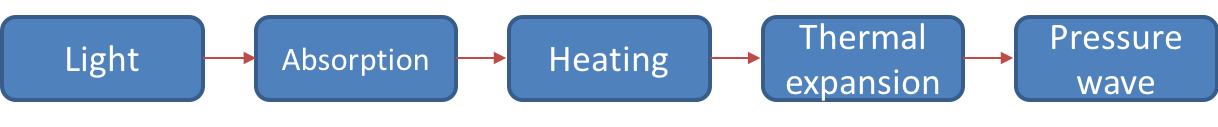
\includegraphics[width = 0.9\textwidth]{02_principles_of_photoacoustics/images/photoacousticGeneration.png}
	\caption{Sequence of the photoacoustic generation process.}
	\label{fig:PAgen}
\end{figure}

Light, for example a laser beam, hits a sample. The laser power can be written as

\begin{equation}
	P_{laser} = \frac{Q_{laser}}{\tau_{laser}}
	\label{eq:LP}
\end{equation}
\\
where $Q_{laser}$ is the laser pulse energy and $\tau_{laser}$ is the pulse duration. With the illuminated area $A_{laser}$ given by the laser beam diameter $d_{laser}$ follows the irradiance 

\begin{equation}
I_{laser} = \frac{4 \cdot P_{laser}}{d_{laser}^2 \cdot \pi} = \frac{P_{laser}}{A_{laser}}
\label{eq:ILaser}
\end{equation}
\\
it is assumed, that the sample surface is much bigger than the illuminated area. 

\begin{figure}[H]
	\centering
	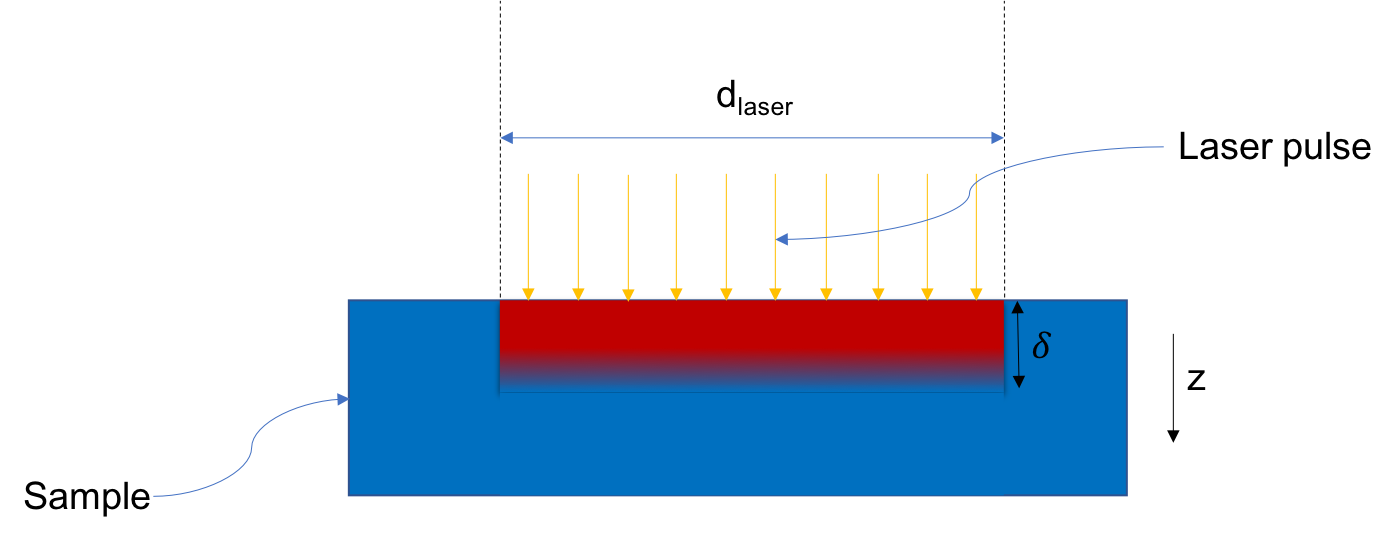
\includegraphics[width = 0.9\textwidth]{02_principles_of_photoacoustics/images/lpOnSample.png}
	\caption{Schematic view of a laser pulse hitting a sample.}
	\label{fig:LPonSample}
\end{figure}

The description of the absorption that happens subsequently is given by the Lambert-Beers law \cite{demtroder:ExPhysik}. Therefore, the depth profile of the irradiated intensity is defined by

 \begin{equation}
 	I(z) = I_{laser}  \cdot exp(-\mu_a \cdot z)
 	\label{eq:lambertbeer}
 \end{equation}
\\
where $\mu_a$ is the optical absorption coefficient of a non-scattering material. It describes the weakening of an incident electromagnetic wave. Furthermore, a penetration depth $\delta = \frac{1}{\mu_a}$, shown in Figure \ref{fig:LPonSample}, is defined by the intensity drop of $\frac{1}{e}$.\\
In the next step the absorbed light is converted into mechanical stress. For non-fluorescent materials it can be supposed, that the whole electromagnetic energy is converted into thermal energy and if the following two conditions are fulfilled, this energy will form an acoustic wave.\\
Whenever the energy is confined into the irradiated volume and does not vanish due to heat conduction, the "heat confinement" is achieved. This means that the laser pulse $\tau_{laser}$ is shorter than the thermal relaxation time $\tau_{th}$
given by
\begin{equation}
	\tau_{laser} < \tau_{th} = \frac{\delta'^2}{4\cdot\lambda_t} 
	\label{eq:thConf}
\end{equation}
\\
where $\delta'$ is the smallest dimension of the illuminated volume (laser beam diameter or penetration depth) and $\lambda_t$ is the thermal diffusivity. \newline
The second requirement for an efficient photoacoustic excitation process is to fulfill the condition for “stress confinement” defined by

\begin{equation}
t_{laser} < t_{ac} = \frac{\delta'}{c_s} 
\label{eq:stressConf}
\end{equation}
\\
where $c_s$ is the speed of sound in the medium. This condition ensures that no acoustic relaxation occurs during the excitation process. In either case (heat or stress confinement) a pressure rise, in reference to the equilibrium pressure, is achieved \cite{GrattSibylle:Dis}. 

\begin{equation}
\Delta p = - B \frac{\Delta V}{V}  + B \beta \Delta T
\label{eq:dV/V}
\end{equation}
\begin{equation}
B = \rho_0 c_s^2
\end{equation}
\\
where $B$ is the bulk modulus, $\rho_0$ the density at ambient pressure and $\beta$ the volume expansion coefficient. \\
Due to a laser excitation, the fractional volume expansion is negligible. From this follows an initial pressure rise of

\begin{equation}
p_0 =  B \beta \Delta T = \Gamma \mu_a F
\label{eq:p_0}
\end{equation}
\\
with 

\begin{equation}
\Delta T =  \frac{1}{C_V \cdot \rho } \cdot F \cdot \mu_a 
\label{eq:deltaT} 
\end{equation}
\begin{equation}
\Gamma =  \frac{B \cdot \beta}{\rho \cdot C_V} = \frac{\beta \cdot c_s^2}{C_P}
\end{equation}
\\
$F$...Fluence [J/m$^2$]\\
$C_V$...Heat capacity at constant volume [J/K]\\
$C_P$...Heat capacity at constant pressure [J/K]\\
$\rho$...Density [kg/m$^3$]\\
$\Gamma$...Grueneisenparameter\\\\

The Grueneisenparameter is temperature dependent.  Its property is discussed in chapter \ref{sec:GReffect}. The initial pressure rise relaxes and spreads out as an ultrasonic wave, which can be detected by an ultrasonic transducer \cite{GraflMonika2015Pm, doi:10.1021/cr010436c, WangLihongV2012BO:P}.

\subsection{Generation and propagation of photoacoustic waves}

The general photoacoustic equation is \cite{Wang:PAMtutorial}

\begin{equation}
	\left( \nabla^2 - \frac{1}{c_s^2} \frac{\partial^2}{\partial t^2}\right)p(\vec{r},t) = - \frac{\beta}{\kappa c_s^2}\frac{\partial^2T(\vec{r},t)}{\partial t^2}
	\label{eq:generalPA}
\end{equation}

with

\begin{equation}
	\kappa = \frac{C_P}{\rho c_s^2 C_V}
\end{equation}
\\
where $T$ is the temperature rise, $\kappa$ the isothermal compressibility and $p(\vec{r},t)$ the acoustic pressure at position $\vec{r}$ and time $t$. Equation \ref{eq:generalPA} contains a source term on the right side and a wave propagation term on the left.\\
If a laserpulse fulfills the terms for heat and stress confinement the heating function can be expressed as

\begin{equation}
	H(\vec{r},t) = \rho C_v \frac{\partial T(\vec{r},t)}{\partial t} = \mu_a F
\end{equation}
\\
This follows with equation \ref{eq:generalPA} and the source term, in this case $H$, a time derivative related equation. 

\begin{equation}
		\left( \nabla^2 - \frac{1}{c_s^2} \frac{\partial^2}{\partial t^2}\right)p(\vec{r},t) = - \frac{\beta}{C_p}\frac{\partial H(\vec{r},t)}{\partial t}
\end{equation}
\\
Therefore, only time-variant heating produces a pressure wave. The general photoacoustic equation \ref{eq:generalPA} can be solved by the Green's function approach. This leads to

\begin{equation}
	p(\vec{r},t) = \frac{\beta}{4 \pi C_p} \int \mathrm{d} \vec{r}\,^{'} \frac{1}{\vert \vec{r} - \vec{r}\,^{'} \vert} \frac{\partial H(\vec{r}\,^{'}, t^{'})}{\partial t^{'}} \Bigg|_{ t^{'}=t-\frac{\vert \vec{r}-\vec{r}\,^{'} \vert}{c_s}}
\end{equation} 
\\
where $\vec{r}\,^{'}$ and $t^{'}$ are the location and time  of the source. If $H(t^{'}) = \delta (t^{'})$, $p(\vec{r},t)$ can be written as

\begin{equation}
	p(\vec{r},t) = \frac{1}{4 \pi c_s^2} \frac{\partial}{\partial t} \left[ \frac{1}{c_s t} \int \mathrm{d}\vec{r}\,^{'} p_0(\vec{r}\,^{'}) \delta \left(t-\frac{\vert \vec{r} - \vec{r}\,^{'}\vert}{c_s}\right)\right]
	\label{eq:PAgenArb}
\end{equation}
\\
the square brackets yield a step heating response to an arbitrary absorbing object and its time differentiation follows the delta-heating response. Equation \ref{eq:PAgenArb} can be used to calculate photoacoustic pressure, generated by an heterogeneous optically absorbing object \cite{Wang:PAMtutorial}.\\

\subsubsection{Spherical-source solution and point detector}

The solution for a absorbing spherical object with radius $R_s$, that is homogeneously heated by a delta pulse is

\begin{equation}
p(r,t) = p_0 \left[\theta(R_s - c_s -r) + \frac{r-c_s t}{2r} \theta(r-\vert R_s - c_s t\vert) \theta(R_s + c_s t - r)\right]
\label{eq:prt}
\end{equation}
\\
where 

\begin{equation}
\theta(z) =
\begin{cases}
1 &  \mathrm{for}~z \geq 1\\
0 & \mathrm{else}
\end{cases}
\label{eq:theta}
\end{equation}
\\
the origin of $r$ is the center of the sphere. For an initial pressure of

\begin{equation}
p_0(r) = p_0\theta(r)\theta(-r + R_s);\;\;\;with~ 0\le r < R_s
\end{equation}
\\
formula \ref{eq:prt} becomes

\begin{equation}
p(r,t) = \underbrace{p_0(r+c_st) \cdot \frac{r+c_s t}{2r}}_{\mathrm{I}}+ \underbrace{p_0(-r+c_st) \cdot \frac{r-c_s t}{2r}}_{\mathrm{II}}+\underbrace{p_0(r-c_st) \cdot \frac{r-c_s t}{2r}}_{\mathrm{III}}
\label{eq:p0rt}
\end{equation}
\\
where part I is a converging spherical wave, part II is a radiating spherical wave excited by the converging wave of part I through the center and part III is a radiating spherical wave \cite{Wang:PAMtutorial}.\\
As the converging part I does not propagate outside of the sphere formula \ref{eq:p0rt} reduces into

\begin{equation}
p(z,t) = \frac{z-c_s t}{2z} p_0(-z+c_s t) + \frac{z-c_s t}{2z} p_0(z-c_s t)
\label{eq:p0rtdelta}
\end{equation}
\\
where the pressure wave is detected by a point like ultrasonic transducer, that is placed at distance $z$ outside the spherical source with given source radius $R_s$. \\
Figure \ref{fig:nShape} shows a simulation done with equation \ref{eq:p0rtdelta}.

\begin{figure}[H]
	\centering
	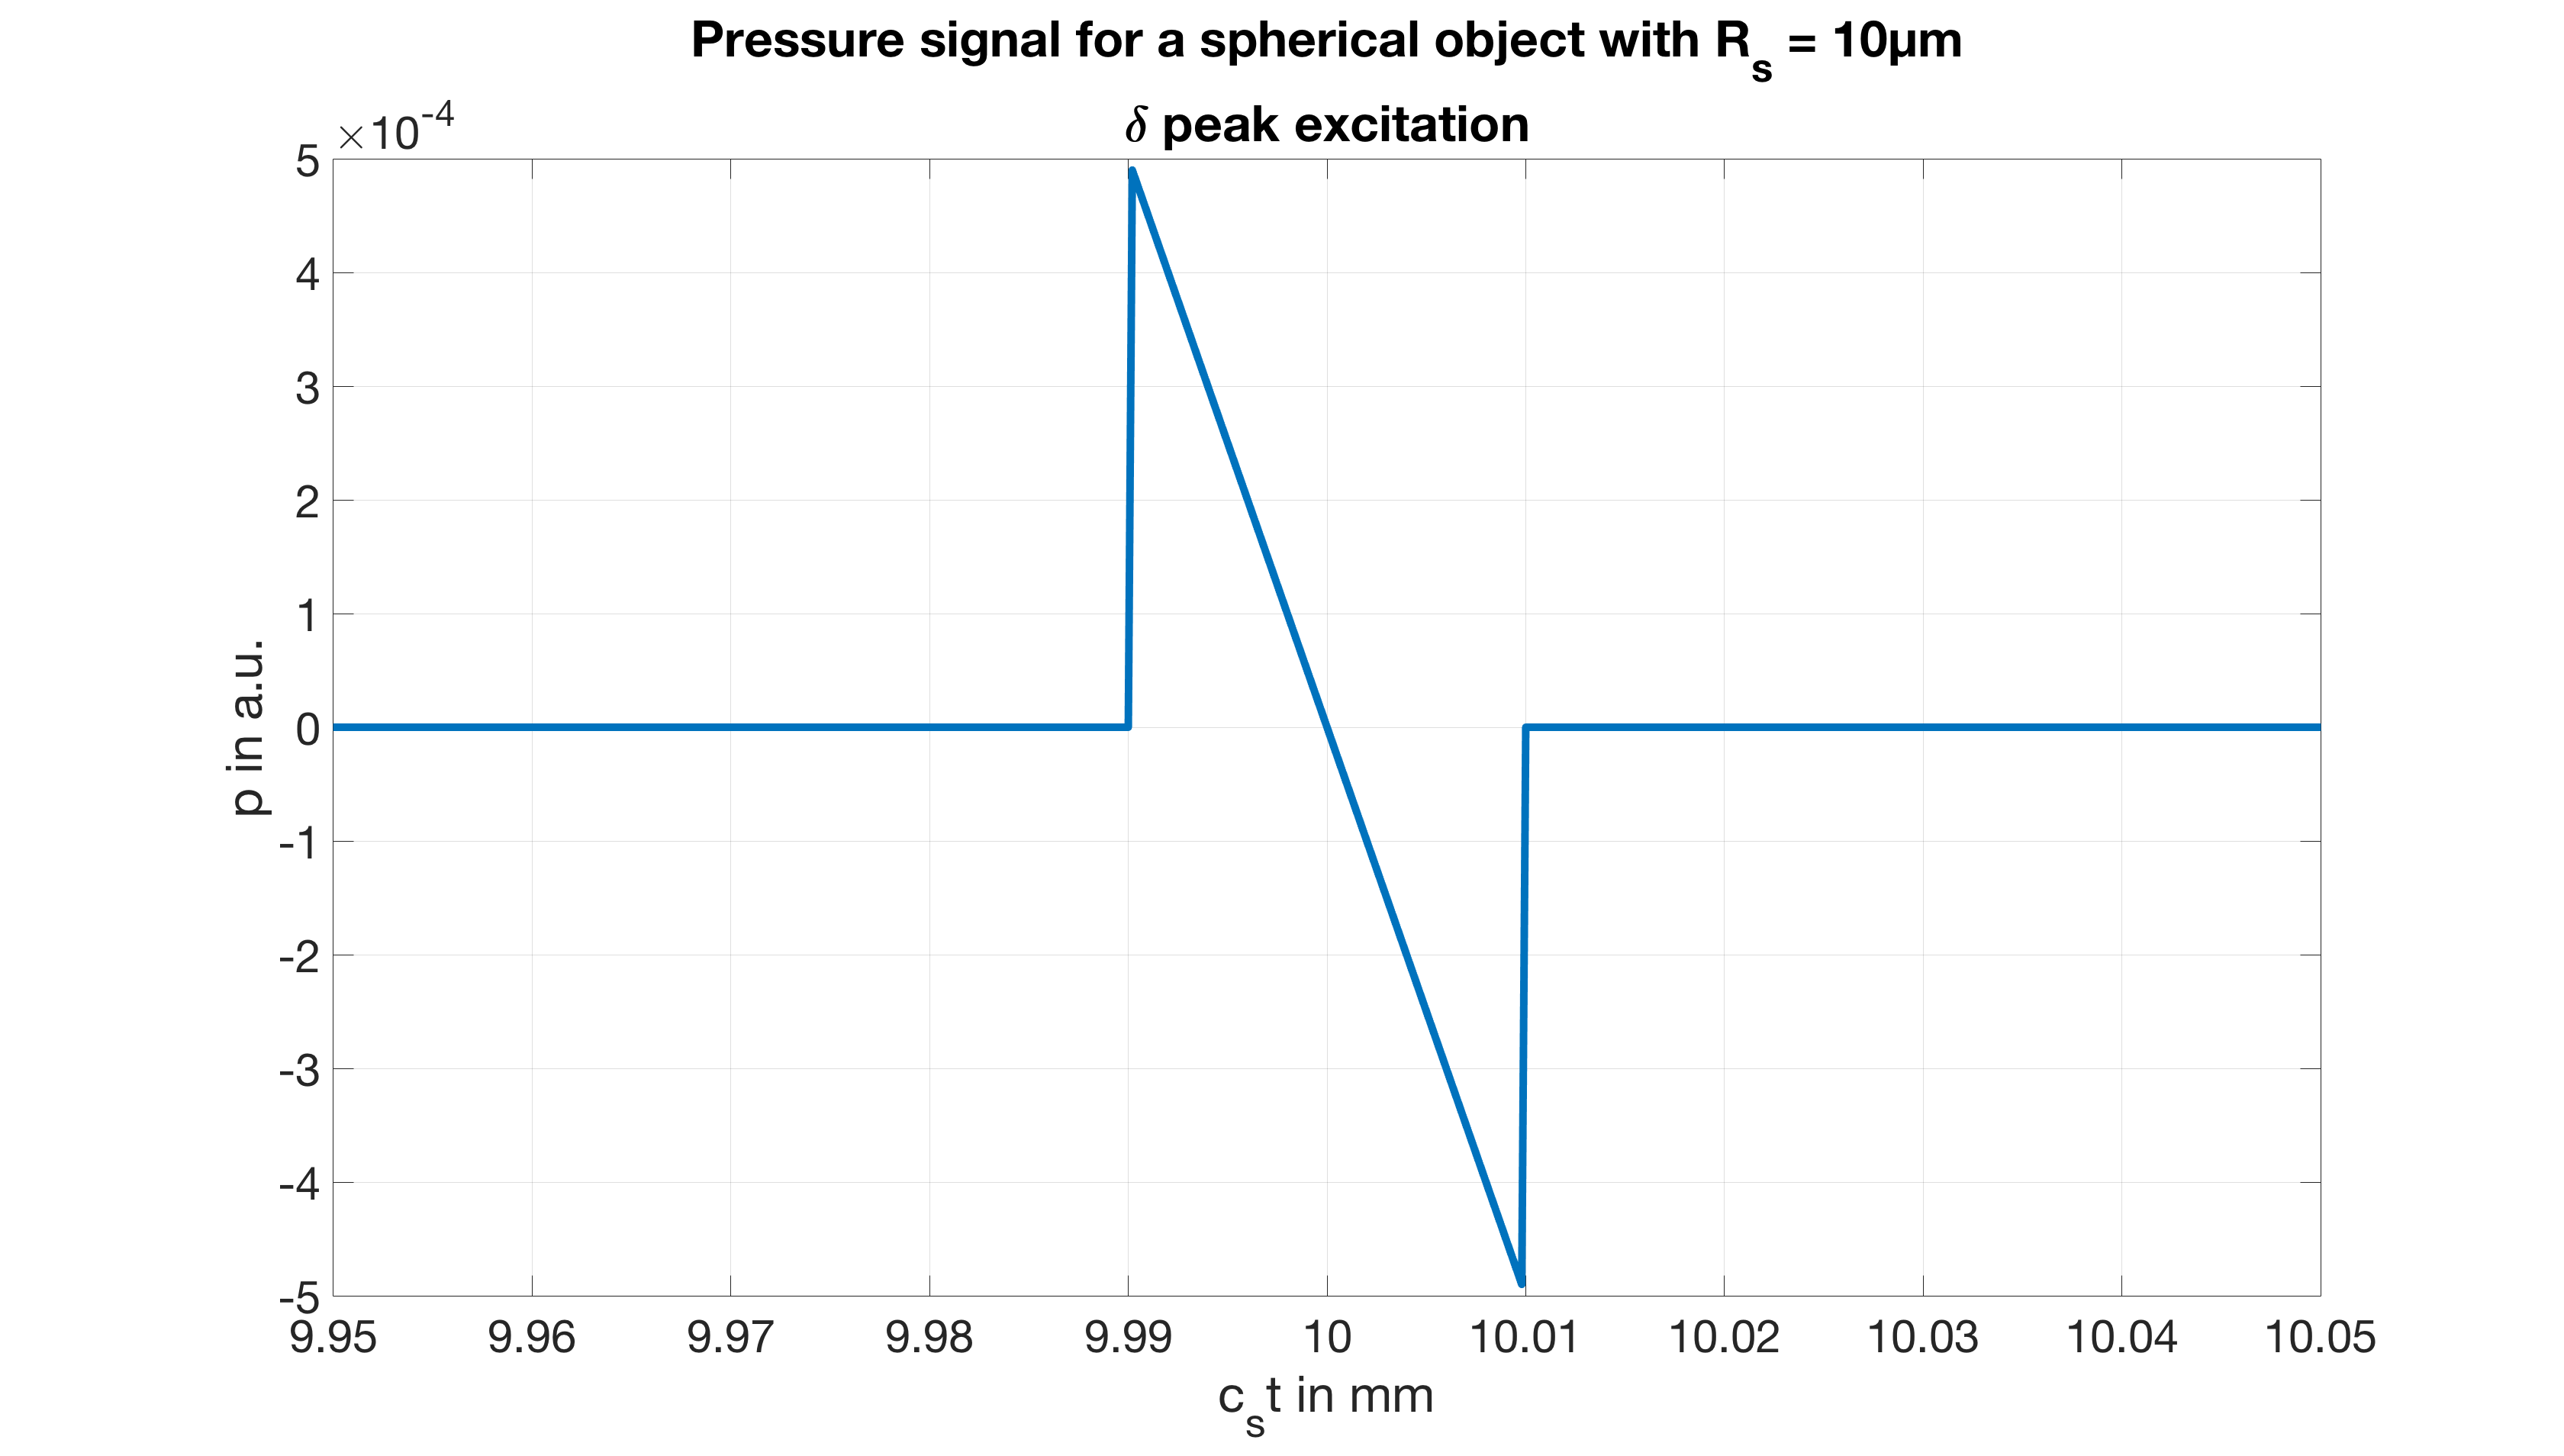
\includegraphics[width = 0.7\textwidth, height=0.3\textheight]{02_principles_of_photoacoustics/images/nShape.png}
	\caption{N-shape signal for a spherical source with $R_s$ = 10~$\mu m$, in $z$ = 10~$mm$ distance and $\delta$ pulse excitation (The calculation program can be found in appendix \ref{app:PAgen}).}
	\label{fig:nShape}
\end{figure}

\subsubsection{Spherical-source solution and finite detector}

The detection of a spherical propagating pressure wave with a pointlike ultrasonic detector corresponds to a convolution of the pressure signal function with a $\delta$-function. Hence the response of a ultrasonic transducer, with finite detection bandwidth, to a spherical pressure wave, can be calculated by a convolution of their time domain functions.\\
In figure \ref{fig:freqTimePAsig} a simulation is done with the parameters given above for the pressure wave excitation. The ultrasonic transducer is modulated by a Gaussian function in the frequency domain, with a center frequency of 50~$MHz$ and 70~$\%$ bandwidth.  

\begin{figure}[H]
	a)
	\begin{minipage}{0.5\textwidth}		
		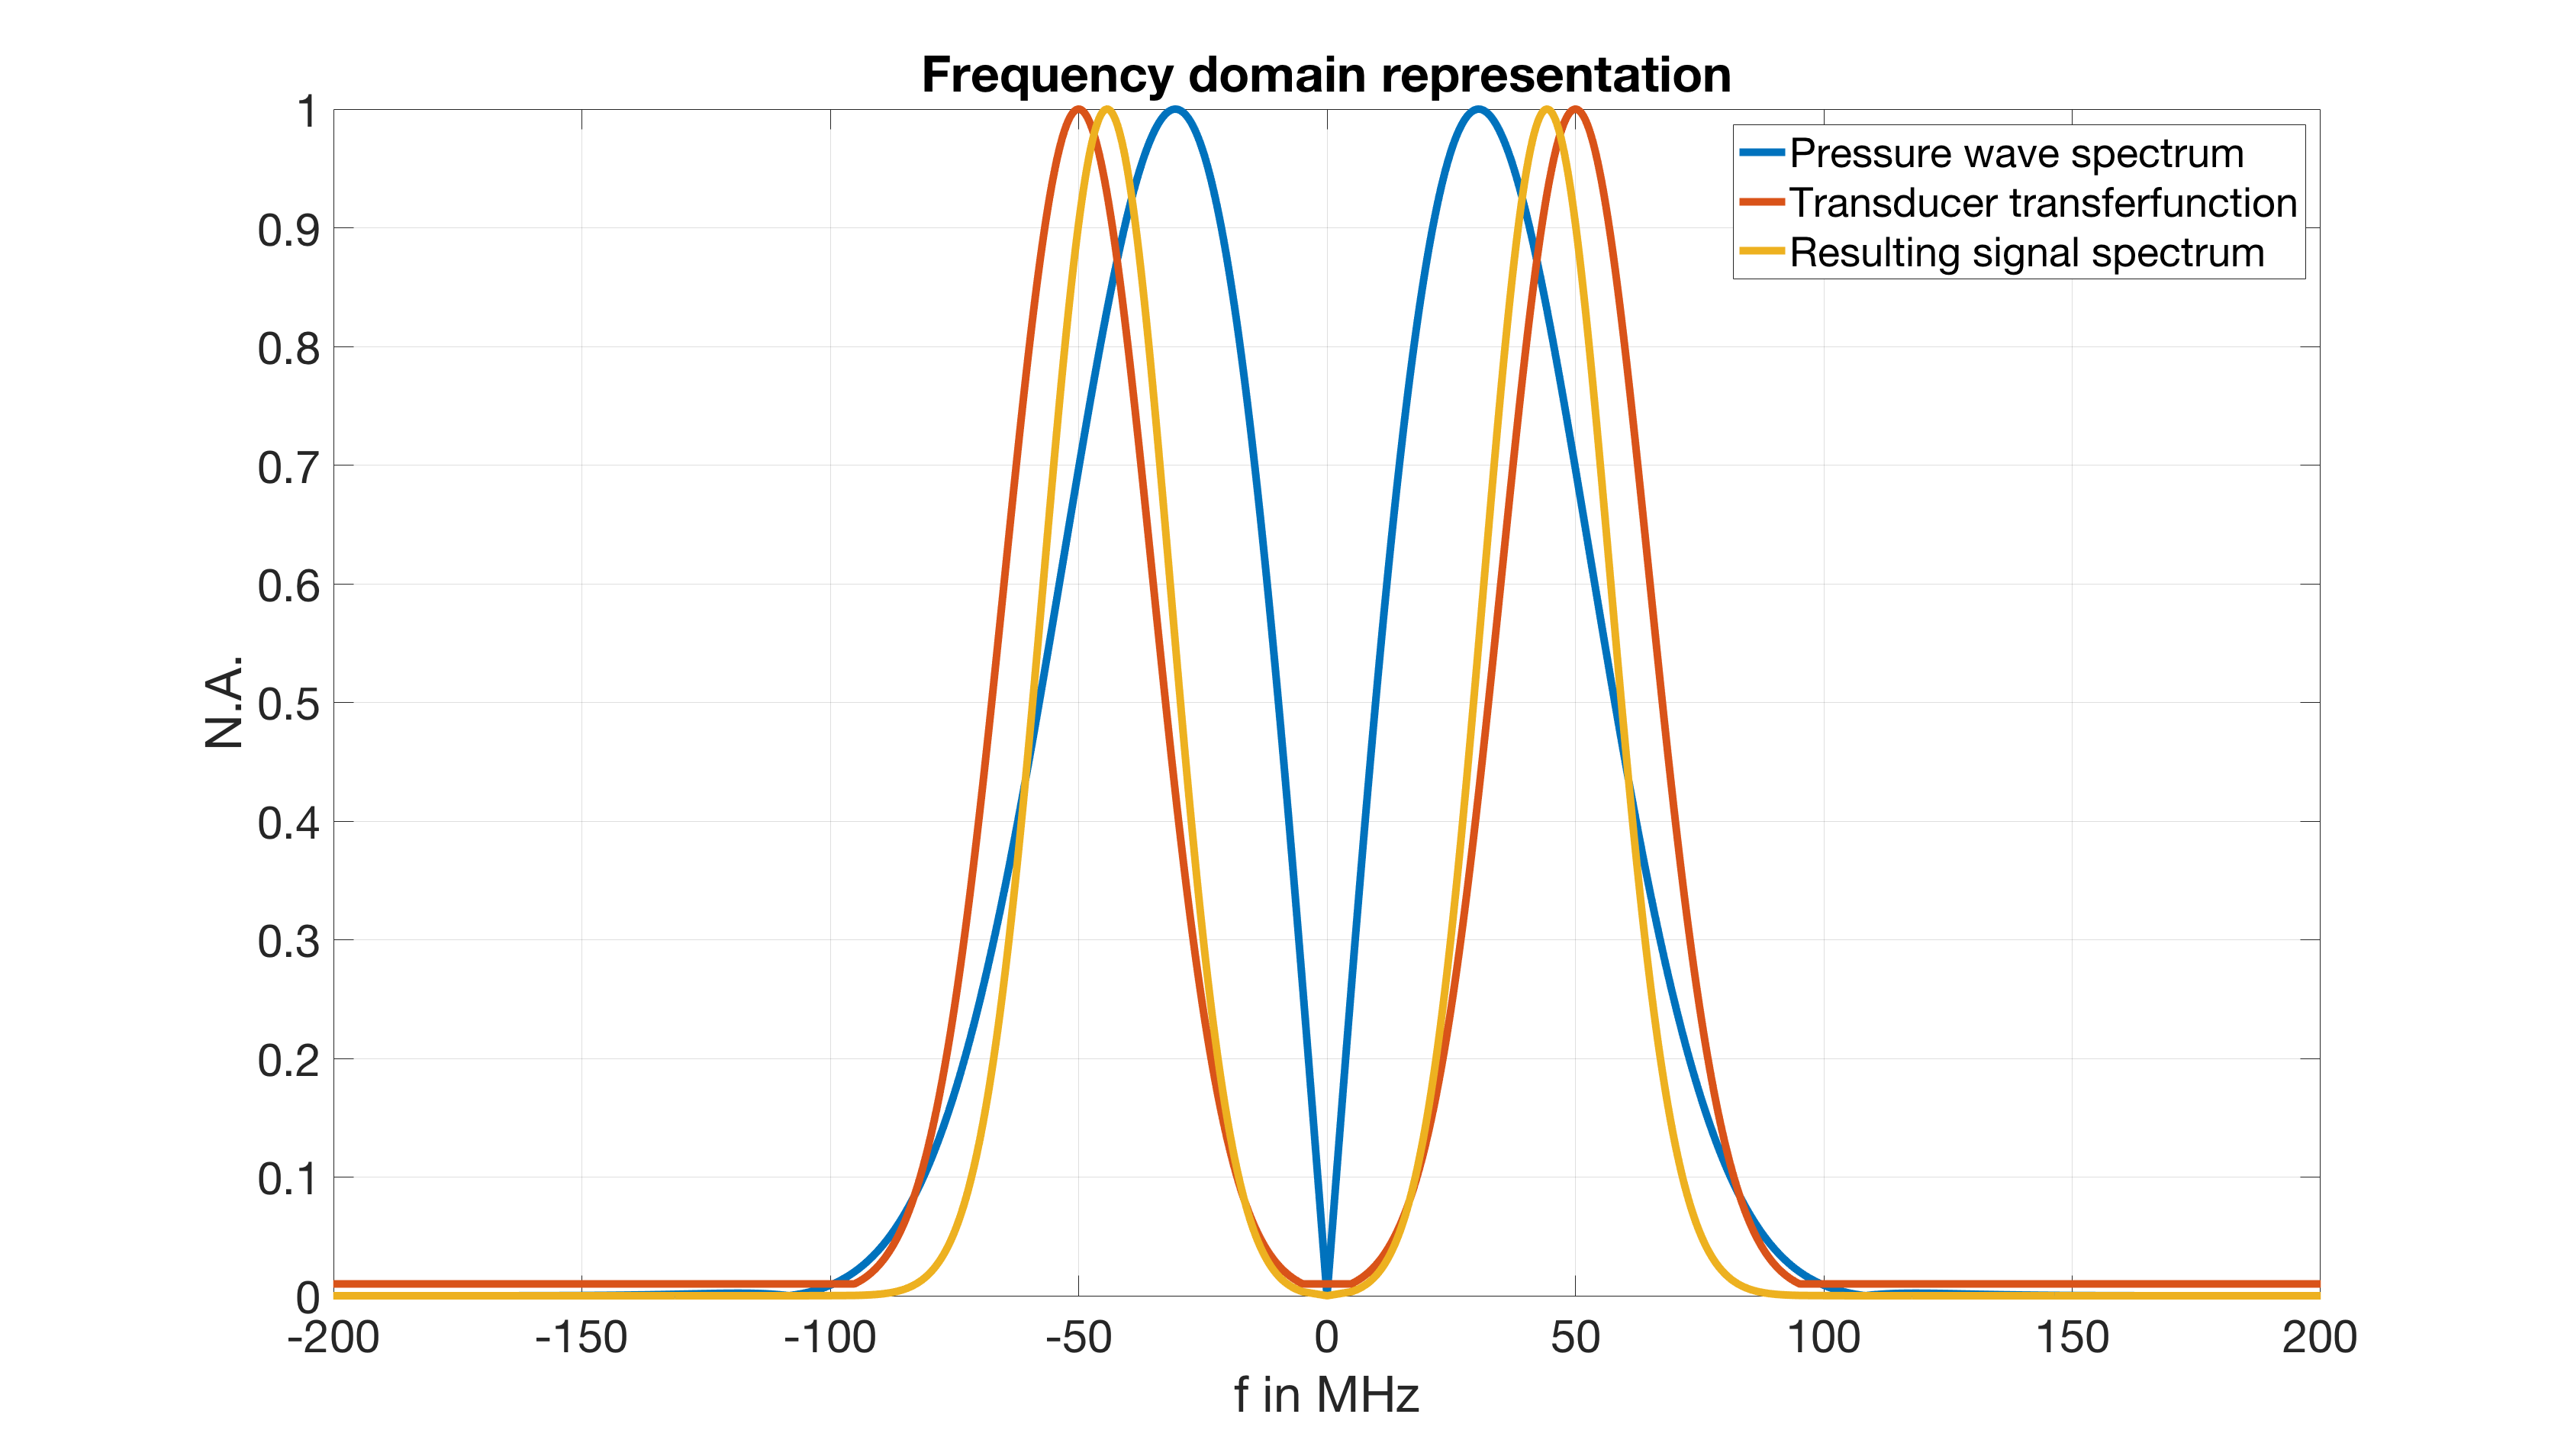
\includegraphics[width = \textwidth, height=0.25\textheight]{02_principles_of_photoacoustics/images/freqSphericalDet.png}
	\end{minipage}
	b)
	\begin{minipage}{0.5\textwidth}		
		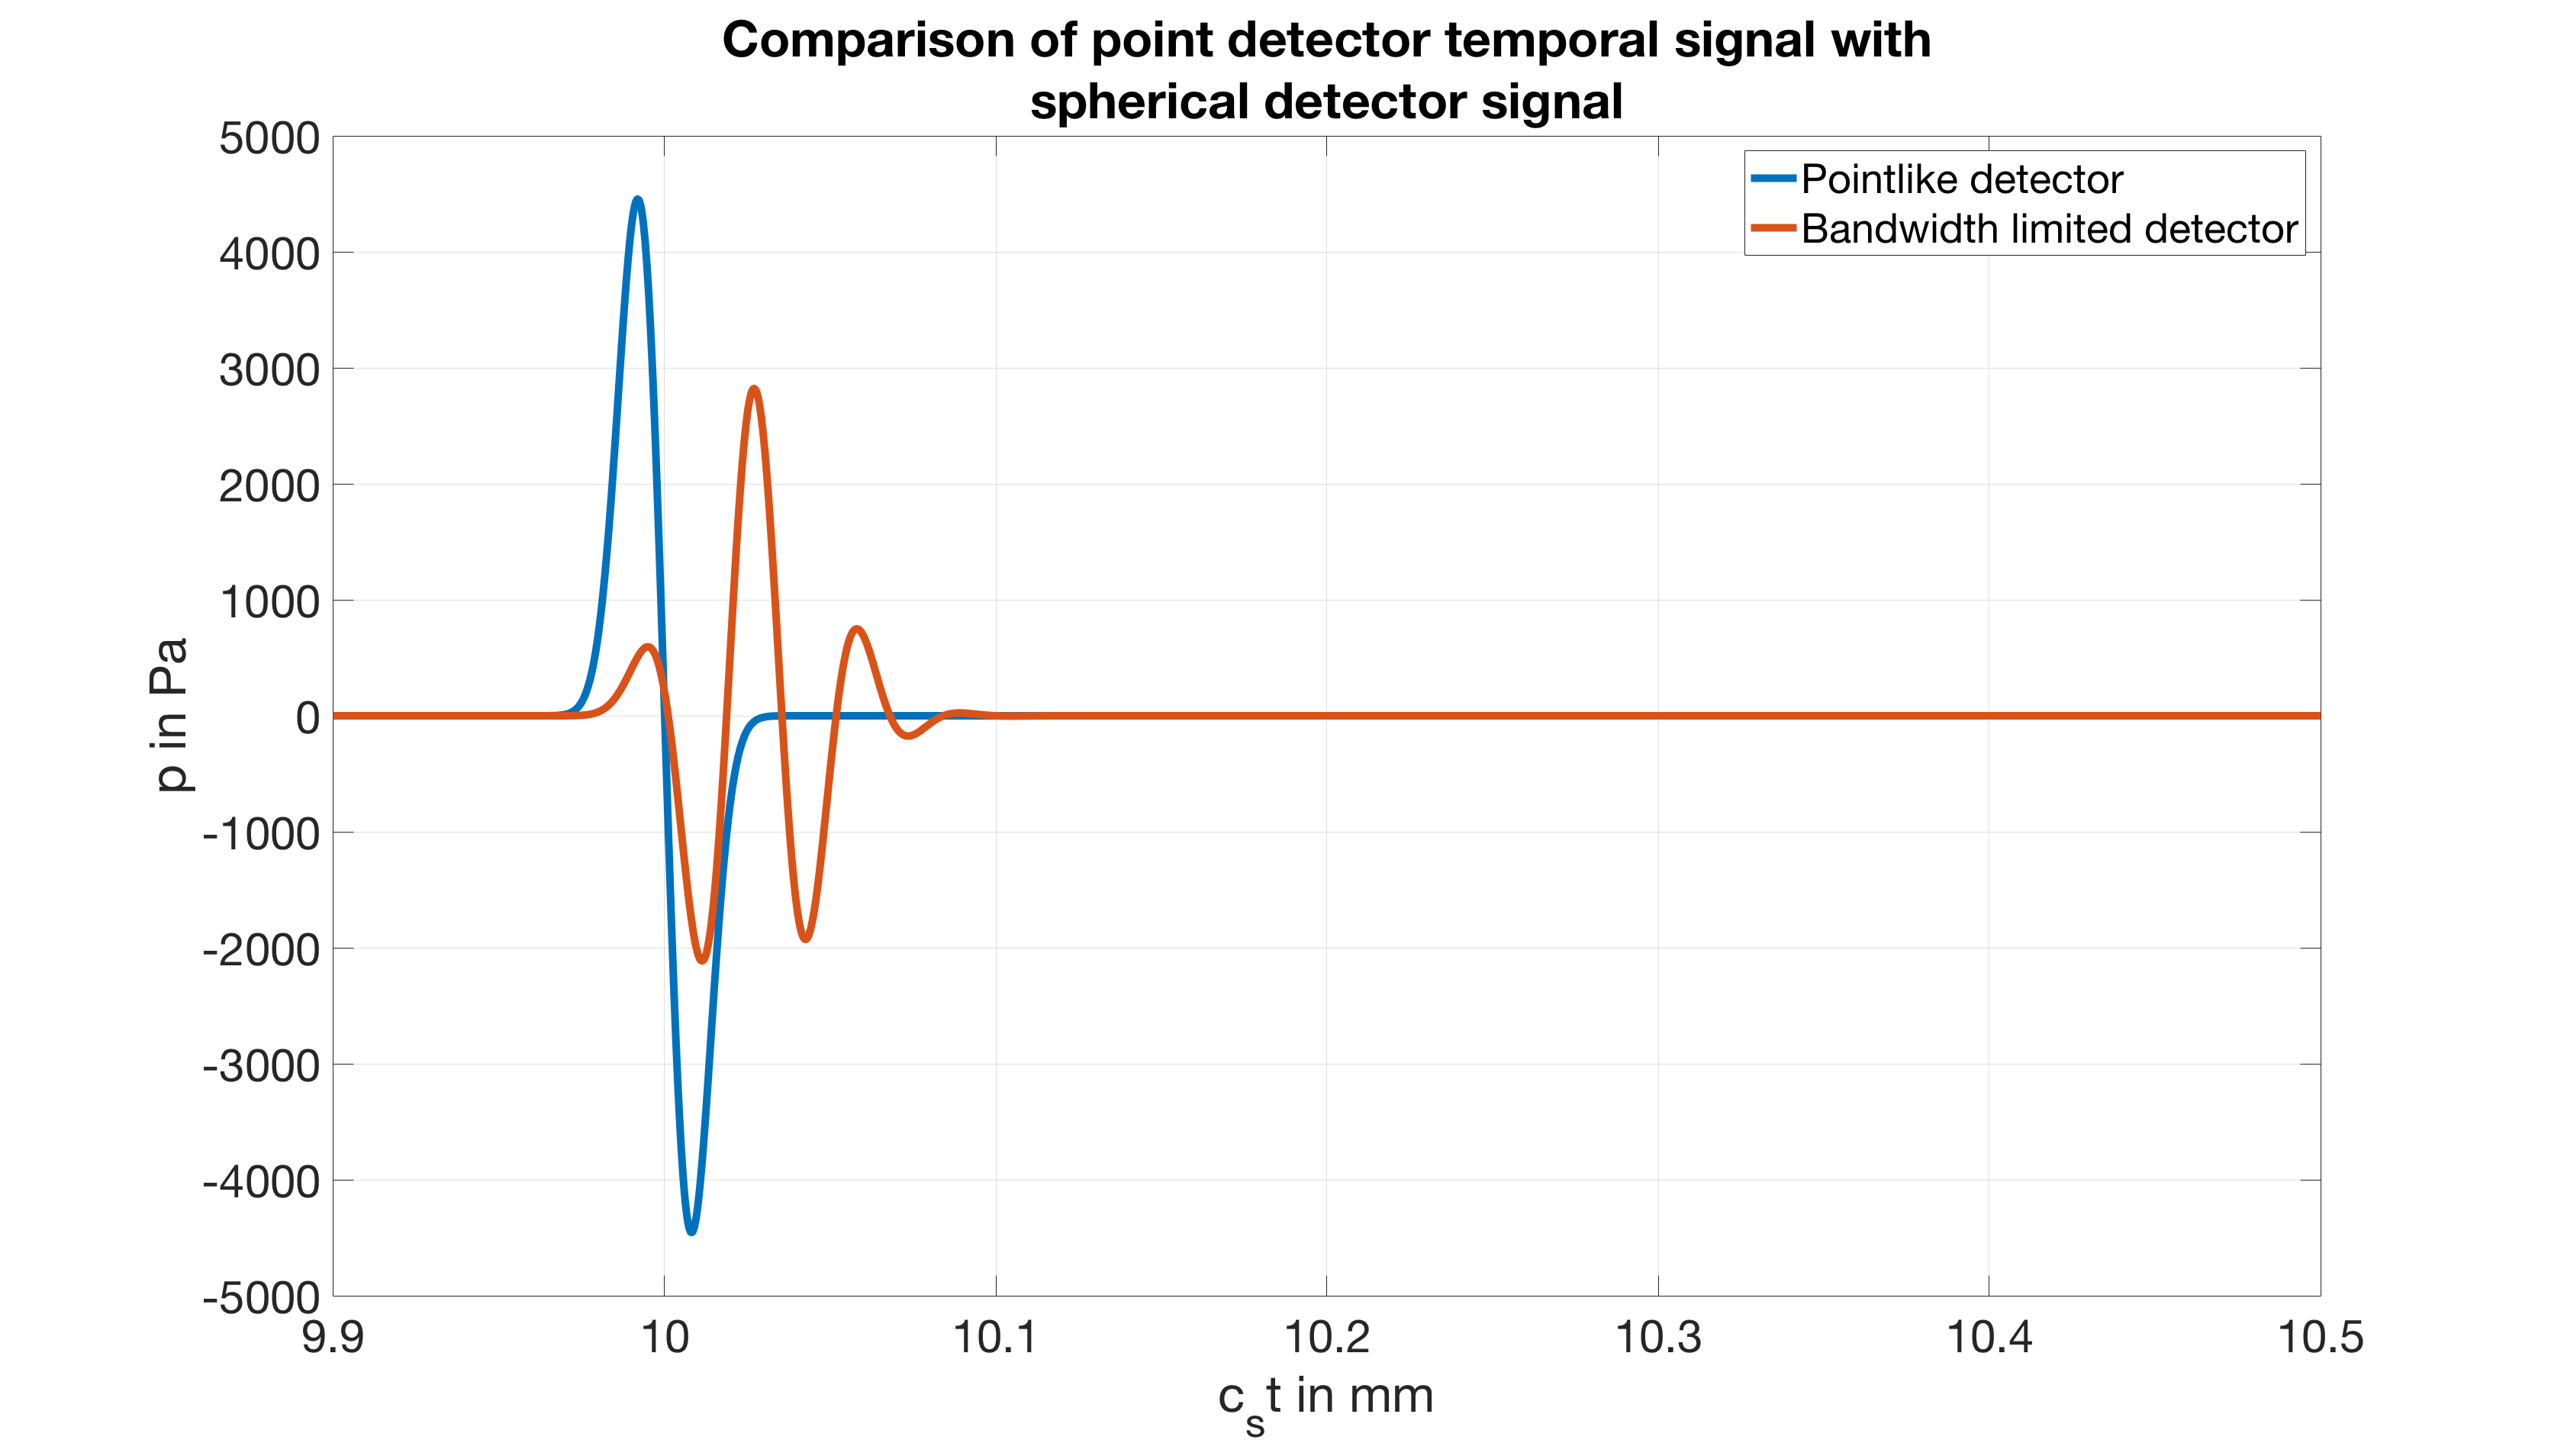
\includegraphics[width = \textwidth, height=0.25\textheight]{02_principles_of_photoacoustics/images/timeSphericalDet.png}
	\end{minipage}	
	\caption{In a) the frequency domain representation of the ultrasonic transferfunction, the source signal function and the resulting signal are shown. The time domain functions, of a pressure wave detected by a pointlike (blue-line) and a bandwidth limited ultrasonic transducer (orange-line), are shown in b). The used code can be found in appendix \ref{app:PAgen}.}
	\label{fig:freqTimePAsig}
\end{figure} 

The simulation clearly shows the impact of the limited bandwidth of the ultrasonic transducer. For comparison, a response function of a real detected signal is shown in figure \ref{fig:PAhilbertSim}. Both show the typical symmetric shape. 

\subsubsection{Study on ultrasonic transducer center frequency}

Based on the previous considerations the impact of the center frequency of a ultrasonic transducer on the maximum amplitude for different source diameter is studied.\\
Three source diameter are studied, 5~$\mu m$, 10~$\mu m$ and 20~$\mu m$. The simulation range for the transducer center frequency is 1 to 100~$MHz$ with a bandwidth of $0.7 \cdot f_{center}$. Therefore not just the value for the center frequency increases, also the bandwidth. The simulation result is shown in figure \ref{fig:centerFreq}.

\begin{figure}[H]
	\centering
	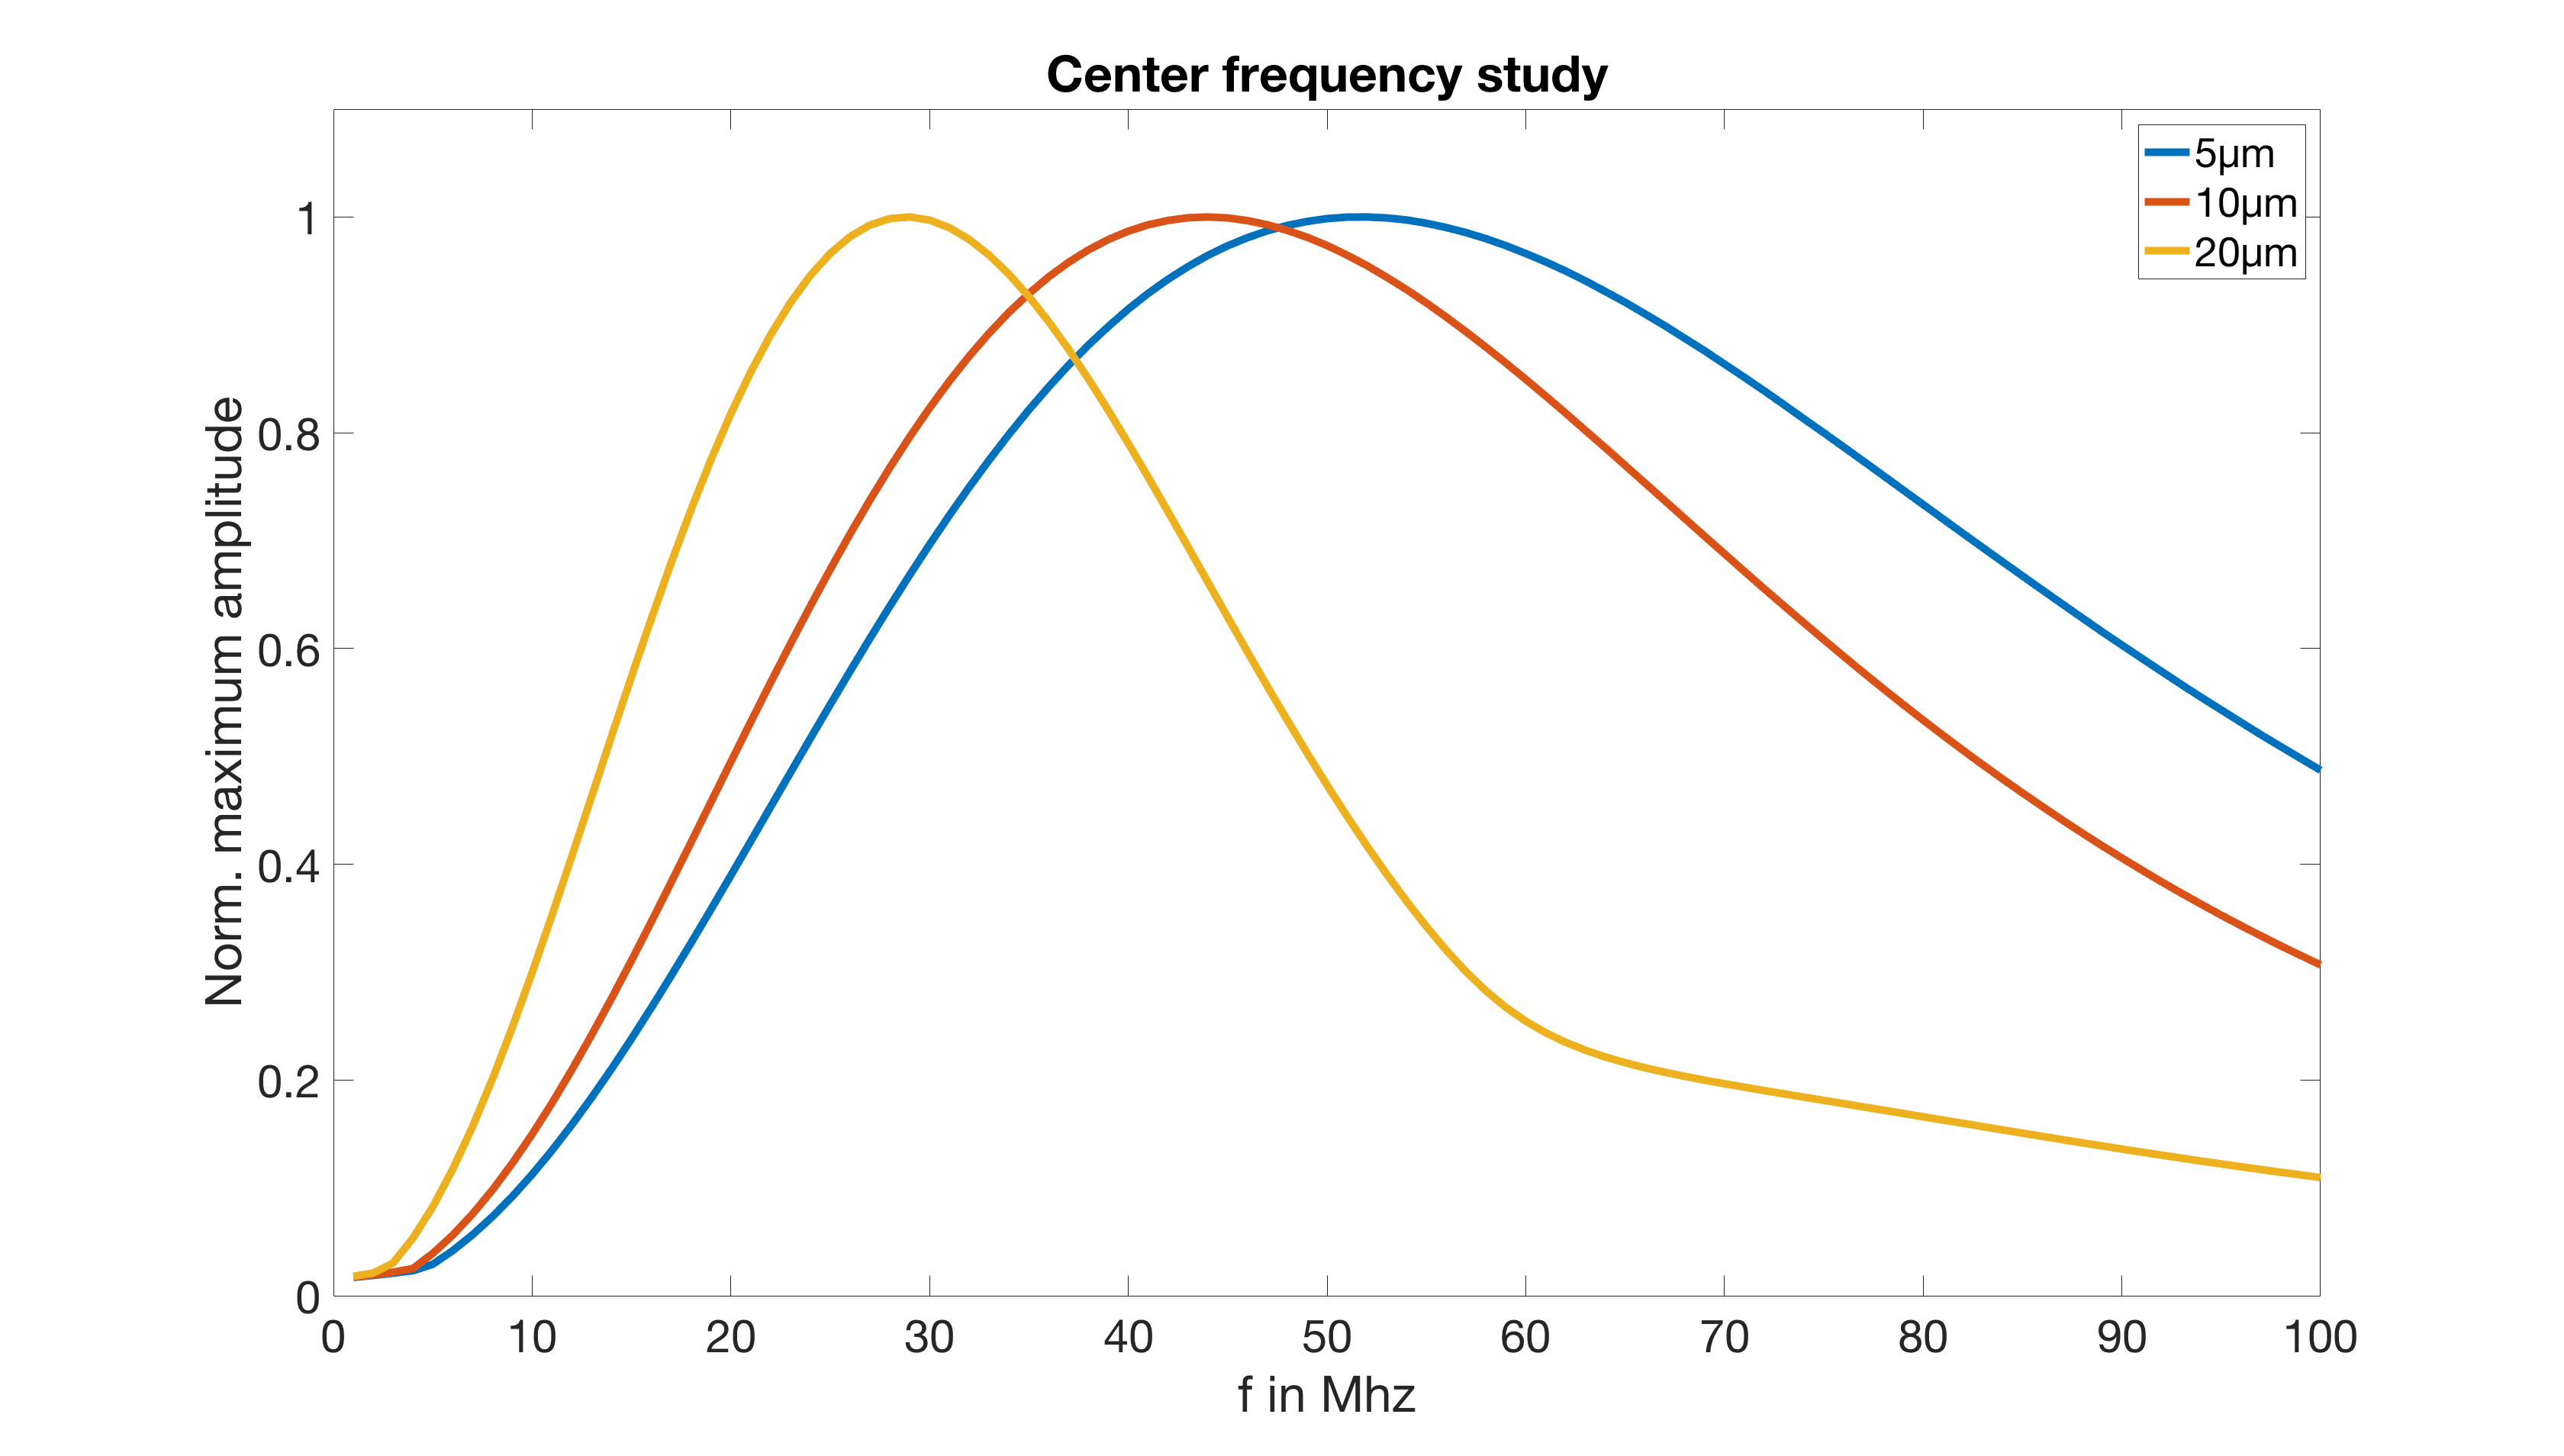
\includegraphics[width = 0.7\textwidth, height=0.3\textheight]{02_principles_of_photoacoustics/images/centerFreq.png}
	\caption{Simulated maximum amplitude response for a 5~$\mu m$, 10~$\mu m$ and 20~$\mu m$ source in dependence of the center frequency of the ultrasonic transducer. The transducers are modeled with a bandwidth of $0.7 \cdot f_{center}$.}
	\label{fig:centerFreq}
\end{figure}

The maximum amplitude values are once more normalized to the maximum possible signal value, for each source diameter.\\
It can be seen that smaller sources produce higher frequency ratios. Therefore it is necessary to use ultrasonic transducer with a high center frequency to image small details.\\
On the other hand the full dimension of bigger sources is only observable if the transducer bandwidth contains lower frequencies, too. For the  20~$\mu m$ source in figure \ref{fig:centerFreq}, a ultrasonic transducer with a center frequency of 29~$MHz$ would be the perfect choice.\\
The source sizes, that should be observed, are in the range of 5 to 10~$\mu m$, therefore a transducer with 50~$MHz$ center frequency and $0.7 \cdot f_{center}$ is chosen.  

\subsection{Photoacoustic microscopy}

On the basis of the photoacoustic effect several applications have emerged. For example microscopy and tomography of biological specimen. \\
In photoacoustic tomography (PAT), the whole area of interest is illuminated. An array of ultrasonic transducers is placed around the sample to receive the excited ultrasonic waves. With the information of how much optical energy was placed onto the sample, the ultrasonic signal coming from different directions and a reconstruction algorithm, a 3D image can be generated. \\
Photoacoustic microscopy (PAM) on the other hand takes one record at a time (A-scan) and generates a picture by scanning over the sample. There are two common methods to do PAM. In acoustical resolution PAM (AR-PAM) a broadened laser beam hits a sample and the generated ultrasonic wave is detected by an ultrasonic detector with focusing properties. The other feasibility is to focus the laser beam onto a sample, so-called OR-PAM, which is discussed in the following, as it is the basis for GR-PAM.

\subsubsection{Optical resolution photoacoustic microscopy (OR-PAM)}

In OR-PAM the optical focus is about a hundred times smaller than the acoustical focus \cite{YAO201487}. A single laser pulse excites an ultrasonic wave with the initial pressure rise given by equation \ref{eq:p_0}. For a PAM in reflection mode, the excited ultrasonic wave propagates back the optical path and is then detected by a ultrasonic transducer. Figure \ref{fig:PAMsetup} shows some possible setups to achieve this configuration. 

\begin{figure}[H]
	\centering
	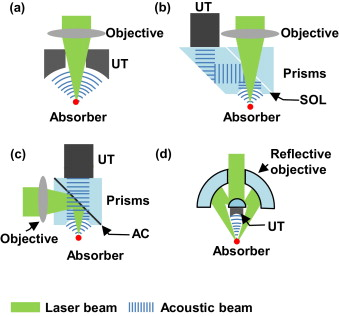
\includegraphics[width = 0.55\textwidth, height=0.3\textheight]{02_principles_of_photoacoustics/images/pamSetups.jpg}
	\caption{Typically used OR-PAM setups. In a) a hole is drilled into the Ultrasonic Transducer (UT), b) uses a silicon oil for refractive index matching (SOL) and therefore generates a optical transparent but acoustical reflective interface, c) is vise versa where the aluminum coating (AC) redirects the laser light and d) uses a reflective objective to focus the light onto the sample \cite{YAO201487}.}
	\label{fig:PAMsetup}
\end{figure}

There are several advantages and disadvantages to every setup.  For example in a), there are losses due to the hole, that have to be drilled into each ultrasonic transducer. In b) and c) the idea is to redirect either the acoustical or the optical pathway. This redirection goes at the expanse of working distance of the applicable objective and therefore the possible Numerical Aperture (NA). In version d) a high NA is possible, but there are losses due to the cable connection for the ultrasonic transducer in the middle. 

\subsubsection{OR-PAM setup}
\label{sec:ORPAMsetup}

The performed measurements were done with the setup shown in Figure \ref{fig:PAMsetup} b). The crucial factor for the choice were the commercial availability of all components used in the setup.\\
For positioning linear stages were used. In x-direction, a PI M-605.2DD controlled by a PI Mercury C-863  and in y-direction a Thorlabs Z825B controlled by a Thorlabs TDC001. The used ultrasonic transducer was an Olympus Panametrics V214-BB-RM with a center frequency of 50~MHz.\\
After the ultrasonic wave is converted into a voltage signal it gets amplified by two Minicircuit ZFL-500LN+ with about 20~$dB$ amplification each. The digitalization is done by a Spectrum M3i.4140-Exp measurement card. Furthermore, the data acquisition and system control is done by a LabVIEW program running on a PC. 

\begin{figure}[H]
	\centering
	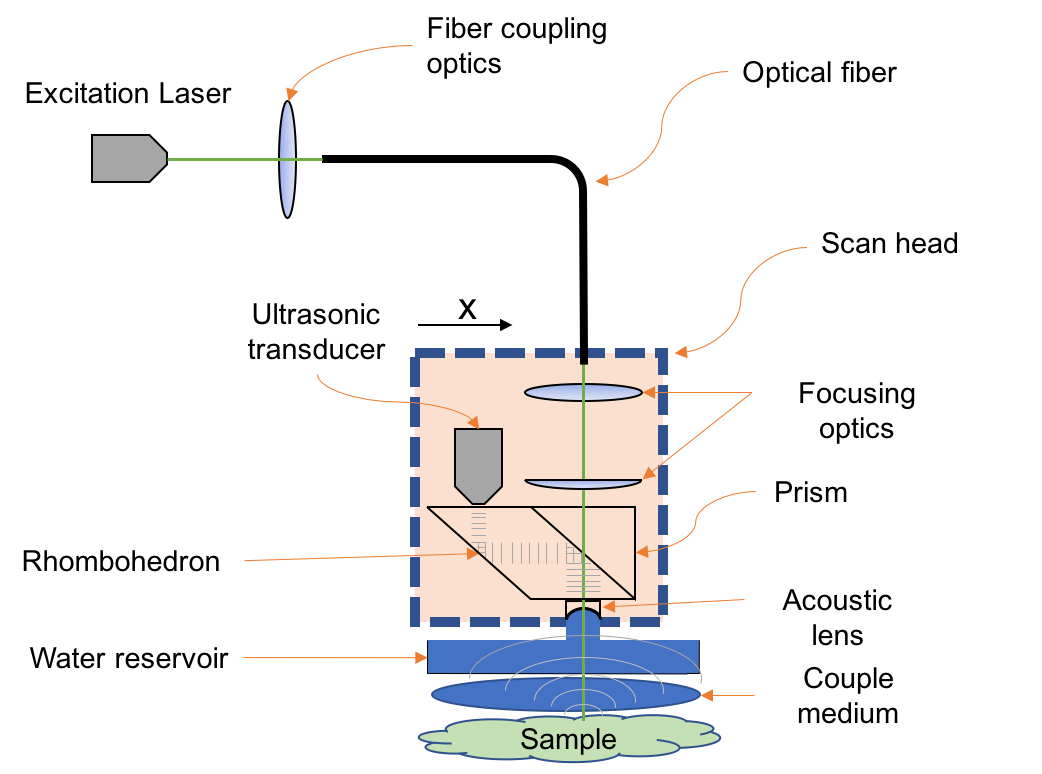
\includegraphics[width = 0.9\textwidth]{02_principles_of_photoacoustics/images/ORPAMsetup.png}
	\caption{Schematic view of the used OR-PAM setup.  }
	\label{fig:ORPAMsetup}
\end{figure}

If the scan head (area, surrounded by the dashed line) is in the right position, the x-direction stage triggers a Quantum Composer 9520 Delay Generator (DG). This device generates a trigger signal for a LCM-DTL-319QT (527 nm) Laser, the measurement card and an oscilloscope that tracks the laser power via a Thorlabs PM100A, with a S120VC photodiode. The laser light is brought to the setup by an optical fiber (Thorlabs P1-460B-FC singlemode, \o = 3.6~$\mu m$).\\
The optical section of the scan head consist of a lens to collimate the laser beam (f = 40~$mm$) and a lens that focuses the light onto the sample (f = 80~$mm$). Acoustically the scan head is coupled to the water reservoir by a water drop that stick at the acoustic lens (45-008 from Edmund Optics), that is glued centered, underneath the rhombohedron prism. The bottom side of the reservoir is made of an acoustical and optical transparent polymer membrane. The sample is acoustically coupled onto the membrane, that restrain the water via a coupling media. Therefore commonly a water droplet is used. \\
The generated ultrasonic wave travels back the optical path. After hitting the acoustic lens the spherical propagating wavefront gets transformed into a plane wave with mostly longitudinal components. The first reflection on the interface between rhombohedron and right-angel prism converts the major part into transversal wave components. In order to properly detected by a piezo electric ultrasonic transducer the signal has to be transformed back into a longitudinal wave, to avoid significant loss of signal strength and information. This is done by a second reflection at the interface (glass/air) on the left side of the rhombohedron prism \cite{Hu:11}. \\
As shown in figure \ref{fig:PAMsetup} b) an index matching liquid is applied to the interface between the rhombohedron and the prism. This ensures that the acoustical wave is deflected on the one hand and the laser beam passes without reflection losses on the other hand. 

\subsubsection{Acoustical runtime considerations}

The time, the ultrasonic wave takes to generate a voltage signal, is important to distinguish between the source signal and the setup reflections. As both reflections come along with mode transformations and therefore differing propagation directions, a detailed investigation were done.\\
In figure \ref{fig:acousticalPath} a closer look onto the setup, described in figure \ref{fig:ORPAMsetup}, is shown. Additionally the estimated acoustic paths, \textit{Path A} and \textit{Path B}, are added.

\begin{figure}[H]
	\centering
	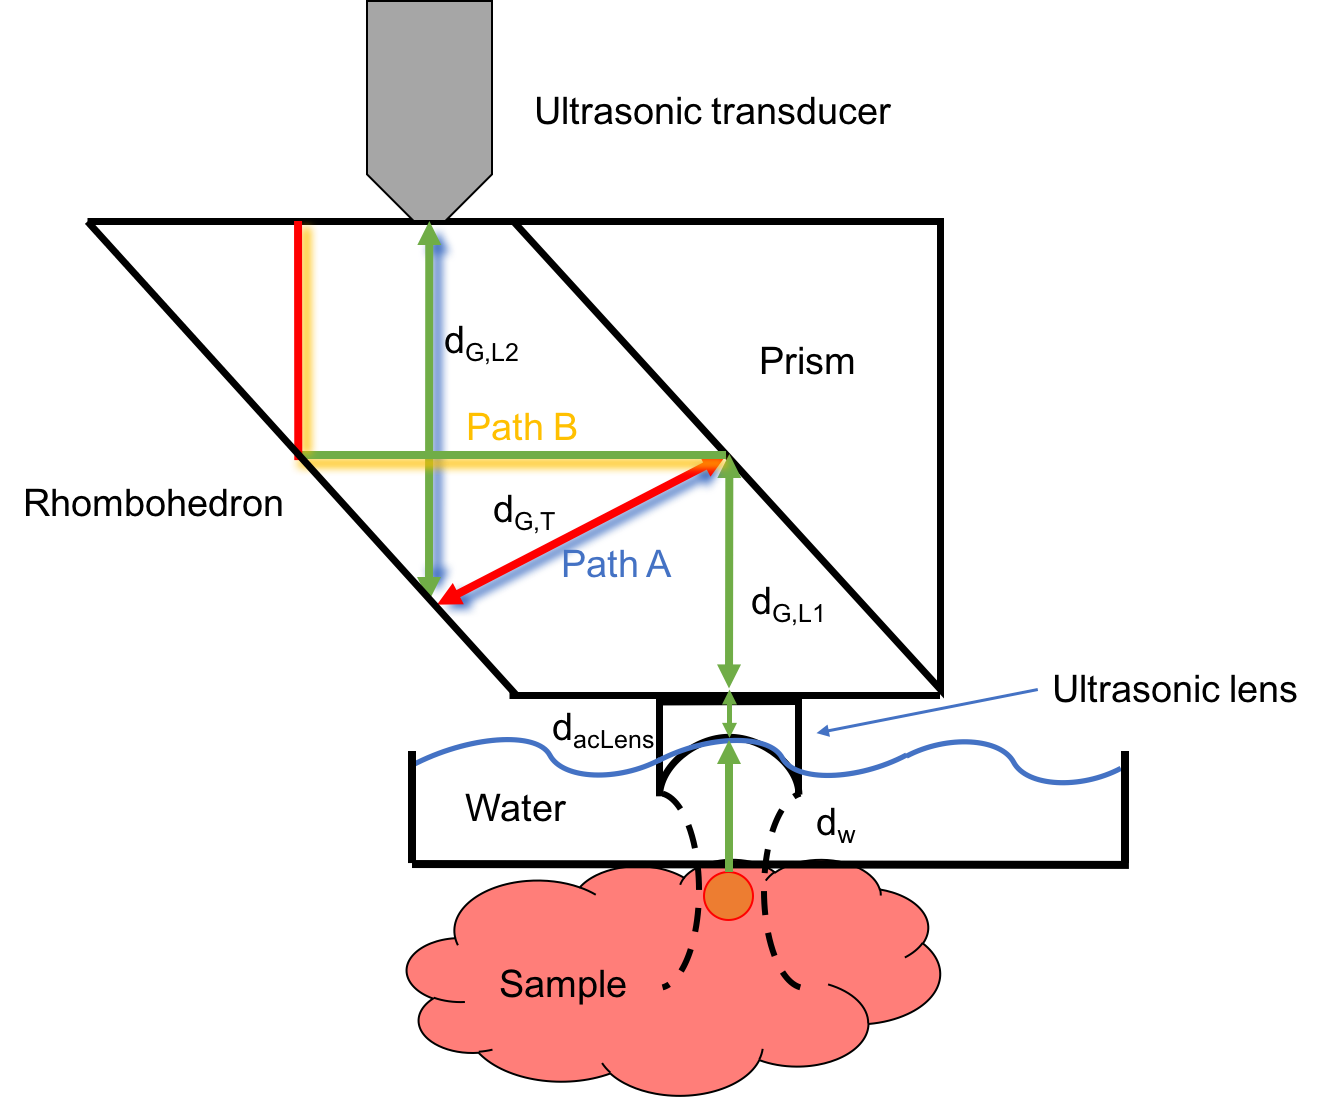
\includegraphics[height = 0.35\textheight, width = 0.6\textwidth]{02_principles_of_photoacoustics/images/ultrasonicPath.png}
	\caption{Zoomed view of figure \ref{fig:ORPAMsetup}. Here the paths taken by the ultrasonic wave are added. The green lines mark longitudinal wave components and the red lines the transversal.}
	\label{fig:acousticalPath}
\end{figure}

The generated ultrasonic wave is a spherical longitudinal wave, which gets transformed into a plane wave by the acoustical lens. As shown in figure \ref{fig:acousticalPath} the longitudinal wave gets mode converted on the right (rhombohedron-prism interface) and the left side (rhombohedron-air interface) of the rhombohedron. The first reflection splits the incident beam into a acoustical \textit{Path A} and \textit{Path B}. Due to the property, of the ultrasonic transducer, to only detect longitudinal modes, the investigated path were \textit{Path A}.\\
For the assumption, that the ultrasonic source object is in the focal plane and the interface between the acoustical lens and the rhombohedron has no impact, the acoustical travel time is 

\begin{equation}
t_{trav} = \frac{d_w}{c_w} + \frac{d_{G,L1}+d_{G,L2}+d_{acLens}}{c_{G,L}} + \frac{d_{G,T}}{c_{G,T}} + t_D
\label{eq:travTime}
\end{equation}
\\
where $d_w$ is the distance the wave travels in water, $d_{G,L1}$ and $d_{G,L2}$ are the longitudinal travel distances in glass and $d_{G,T}$ is the transversal one. The material for the acoustical lens is equal to the rhombohedron material (N-BK7), therefore the speed of sound is the same as for the longitudinal components in glass $c_{G,L}$. Furthermore, the ultrasonic transducer has a delaytime $t_D$. \\
In table \ref{tab:matSpecs} the speed of sound values for the appearing materials are listed.

\begin{table}[H]
	\centering
	\caption{Speed of sound values for N-BK7 and water.}
	\begin{tabular}{| m{2.2cm} | c | c |}
		\hline
		&$c_{longitudinal}$&$c_{transversal}$\\ \hline
		\centering N-BK7 \cite{data:BK7}&6048~$m/s$ &3680~$m/s$\\ \hline
		\centering Water \cite{Haynes:physicalProperties} &1483~$m/s$& - \\ \hline
	\end{tabular}
	\label{tab:matSpecs}
\end{table}

To determine $d_{G,T}$ and $d_{G,L2}$, the behavior of acoustical waves on interfaces is examined. Mechanical waves basically follow Snell's just as optical waves do. \\
In solids a incident longitudinal pressure wave $P_i$, shown in figure \ref{fig:acousticInterface}, transforms into a reflected longitudinal ($P_{P,r}$) respectively transversal part ($P_{T,r}$) and a transmitted longitudinal ($P_{P,t}$) respectively transversal part ($P_{T,t}$), on an interface.

\begin{figure}[H]
	\centering
	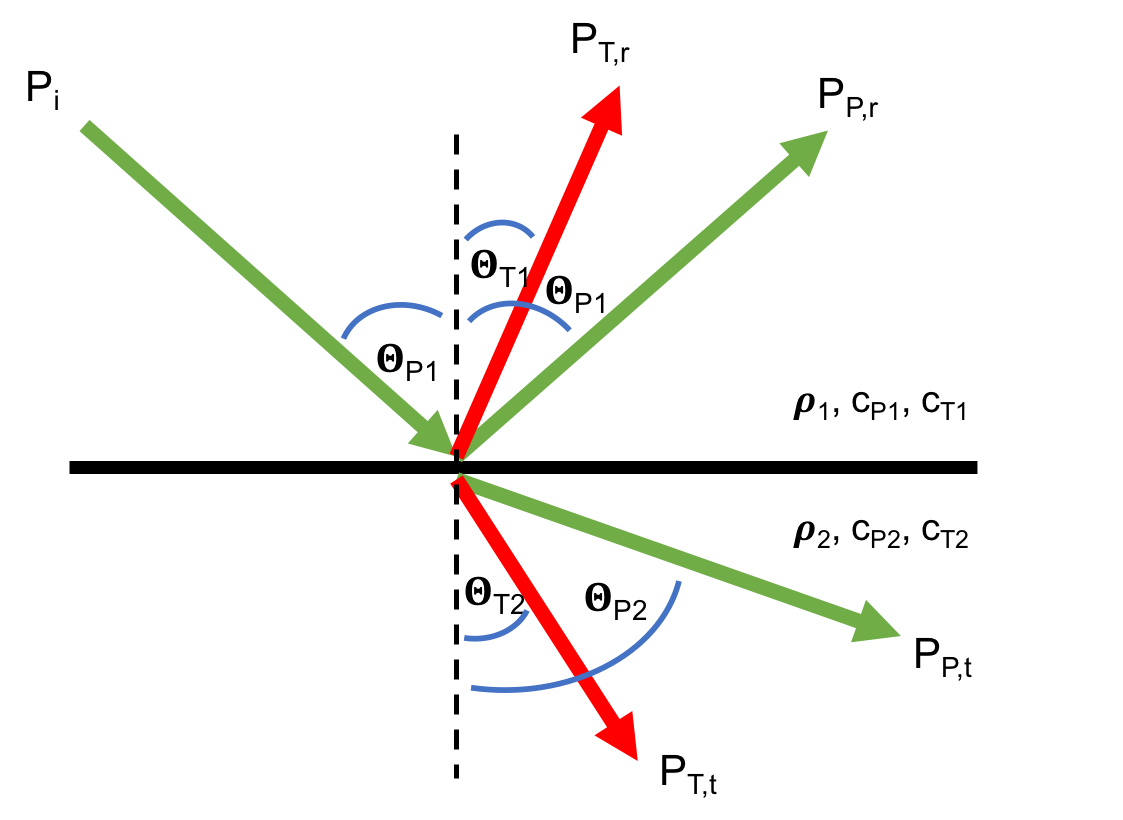
\includegraphics[height = 0.33\textheight, width = 0.58\textwidth]{02_principles_of_photoacoustics/images/acousticInterface.png}
	\caption{Behavior of acoustical waves on interfaces. The longitudinal and transversal wave components are marked with green and red lines.}
	\label{fig:acousticInterface}
\end{figure}

Therefore Snell's law is 

\begin{equation}
	k_{Pi} \sin(\theta_{Pi}) = k_{P_{T,r}} \sin(\theta_{P_{T,r}}) = k_{P_{P,r}} \sin(\theta_{P_{P,r}}) = k_{P_{T,t}} \sin(\theta_{P_{T,t}}) = k_{P_{P,t}} \sin(\theta_{P_{P,t}})
\end{equation}
\\
where k is the wave vector $k_i = \frac{2 \pi f}{c_i}$. \\
The modified lensmaker equation gives the focal length of the acoustical lens and therefore the travel distance for the pressure wave in water \cite{GraflMonika2015Pm}.
\begin{equation}
f_{ac} = d_w = - R \cdot \frac{1}{\frac{c_w}{c_{N-BK7}}-1} = 8.21~mm
\end{equation}
\\
The value for $R$ = 6.2~$mm$ and for $d_{acLens}$ = 1.5~$mm$ (center thickness value) were taken from the 45-008 datasheet \cite{data:45008}.\\
The delaytime of the ultrasonic transducer is 2.15~$\mu s$. The values for $d_{G,T}$ (11.75~$mm$), $d_{G,L1}$ (7.5~$mm$) and $d_{G,L2}$ (11.42~$mm$) are solved by geometrical optics. \\
Inserting into formula \ref{eq:travTime} follows for the acoustical travel time $t_{trav}$ = 14.26~$\mu s$.\\
Signals, which are in the range of $t_{trav}$,  are considered to be generated at the acoustical focal plane.
\pagebreak
\subsubsection{Data acquisition (DAQ) in PAM}
\label{sec:DAQ}

In order to record an image in OR-PAM, a certain sequence have to be executed. \\
At first a field size is defined in the user interface. For example in Figure \ref{fig:scanProcess} a field of view 300 x 300 ($N_x$ x $N_y$) points and a  stepsize of 20~$\mu m$ in both directions are chosen. 

\begin{figure}[H]
	\centering
	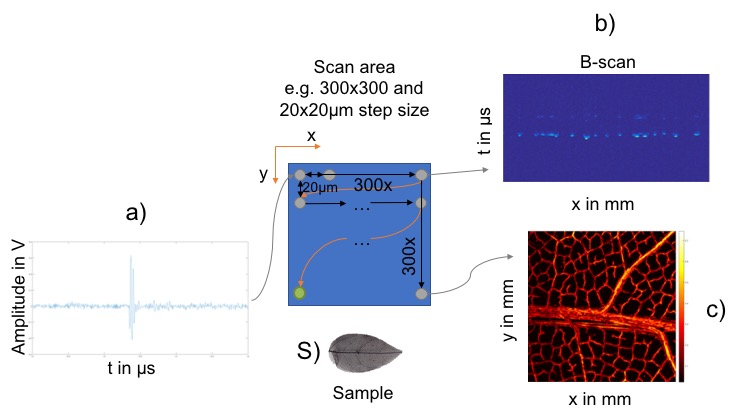
\includegraphics[width = 0.9\textwidth]{02_principles_of_photoacoustics/images/scanProcess.jpg}
	\caption{Illustrated procedure of a scan process. Sample is the black plastic leaf S). a) shows a typical photoacoustic A-scan signal, b) a B-scan image and c) a generated C-scan image, where the maximum of each recorded A-scan is taken.}
	\label{fig:scanProcess}
\end{figure}

In \ref{fig:scanProcess} a) a typical photoacoustic signal is shown, that is called A-scan. At every point in the scan area such a A-scan signal is recorded. As the scan head moves over the sample, every 20~$\mu m$ a detection point is taken. After 300 recorded points in x-direction the scan head moves into the next line. \\
If the 300 A-scan signals are drawn together, a B-scan as shown in \ref{fig:scanProcess} b) is created. A B-scan is termed to be a cut through the sample. The x-coordinate gives the length and the y-coordinate the time-depth (recorded sequence) of the cut.\\
After 300 lines are scanned, a three dimensional cube is created with the size of 

\begin{equation}
	V_{PAcube} = N_x \cdot \Delta x \cdot N_y \cdot \Delta y \cdot t \cdot c_s
\end{equation}
\\
where $t$ is the recorded time interval and $c_s$ the average speed of sound between origin of the ultrasonic wave and the transducer. Based on that several data analysis operations can be executed. For example the maximum amplitude of each photoacoustic amplitude (PA) track, shown in Figure \ref{fig:scanProcess} a), can be extracted and displayed, shown in Figure \ref{fig:scanProcess} c).\\
Furthermore, a topological mapping of the sample is possible due to the runtime information of the ultrasonic signal. This is shown in section \ref{sec:topoPAI}. 

\subsubsection{Hilbert transformation in PAM}

The Hilbert transformation (HT) is an integral transformation equal to the Fourier transformation. In signal processing theory it is used to assign an analytical signal $\hat{x}(t)$ to a real signal $x(t)$. 

\begin{equation}
\hat{x}(t)= x(t) + j \mathcal{H}\{x(t)\}
\end{equation}
\\
An analytical signal is a complex function and has no negative frequencies in its spectrum and is therefore causal. This leads to the property that real and imaginary parts of $\hat{x}(t)$ can be converted into each other, as follows

\begin{equation}
	Re\{\hat{x}(t)\} = - \mathcal{H}\{Im\{\hat{x}(t)\}\}
\end{equation}
\begin{equation}
	Im\{\hat{x}(t)\} =  \mathcal{H}\{Re\{\hat{x}(t)\}\}
\end{equation}
\\
For example, $x(t) = \cos(\omega_0 t)$. The corresponding Hilbert transformed is $\mathcal{H}\{x(t)\} = \sin(\omega_0 t)$ and therefore the analytical signal

\begin{equation}
\hat{x}(t) =  \cos(\omega_0 t) + j \sin(\omega_0 t) 
\end{equation}
\\
the absolute value is $r = \sqrt{\cos(\omega_0 t)^2 +  \sin(\omega_0 t)^2} = 1$ and also the complex envelope of $x(t)$. In figure \ref{fig:PAhilbertSim} this principle were applied to a PA signal \cite{book:girodSystemtheorie}.  

\begin{figure}[H]
	\centering		
	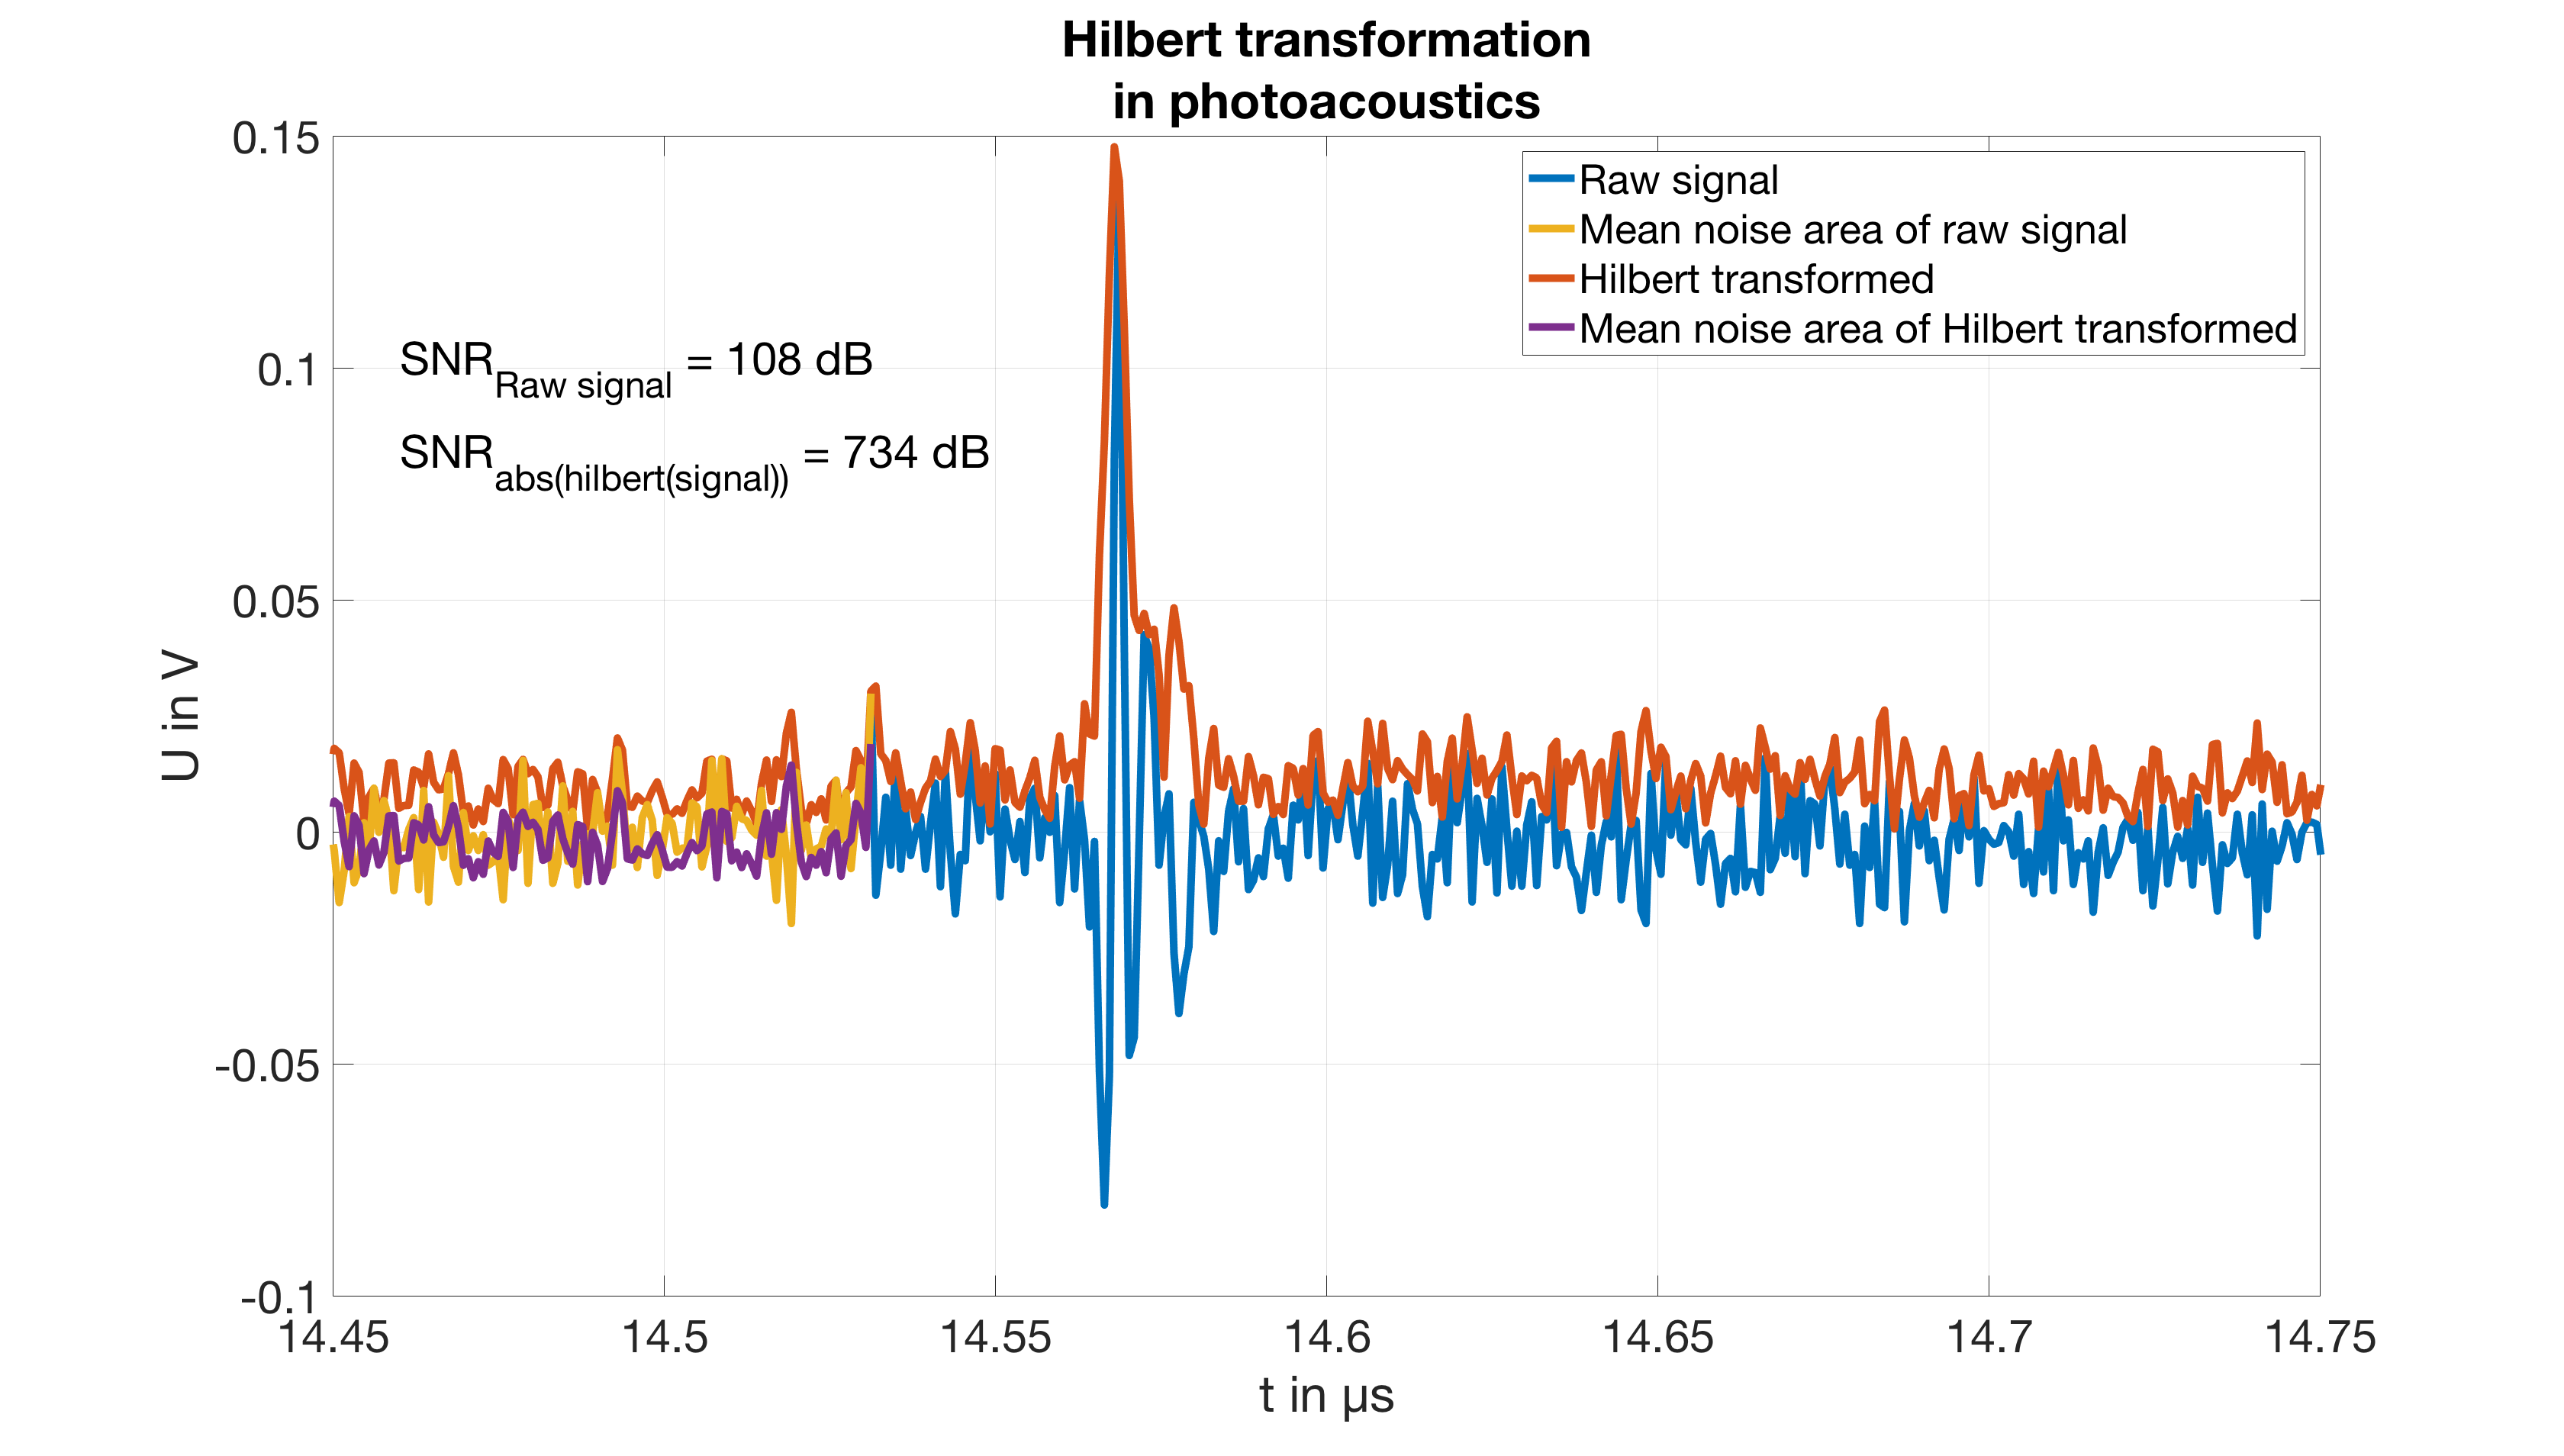
\includegraphics[width = \textwidth]{02_principles_of_photoacoustics/images/measHilbertPA.png}
	\caption{The blue line is the measured PA and its Hilbert transformation in orange. For the signal to noise ratio (SNR) the maximum amplitude of the signals and the mean noise displayed in yellow for the raw signal and purple for the Hilbert transformed. Furthermore, the constant component of the Hilbert transformed were subtracted. }
	\label{fig:PAhilbertSim}
\end{figure}

The blue line is the PA signal and the orange line is the absolute value of its Hilbert transformed. Inside the plot the SNR values for both are shown. For the Hilbert transformed line the value is about seven times higher than the original one.\\
Therefore the HT is a helpful method to suppress noise. The drawback is that the full width at half maximum (FWHM) broadens. As the axial resolution of OR-PAM is determined by the frequency bandwidth of the detecting ultrasonic transducer and thus to the FWHM of the detected signal, the HT reduces the resolution \cite{Ma:GRPAMinVivo}.\\ 
In figure \ref{fig:BsacanHilbert} the difference between a normal B-scan a) and a B-scan, where every detected sequence were Hilbert transformed b), is shown.

\begin{figure}[H]
	a)
	\begin{minipage}{\textwidth}		
		\centering
		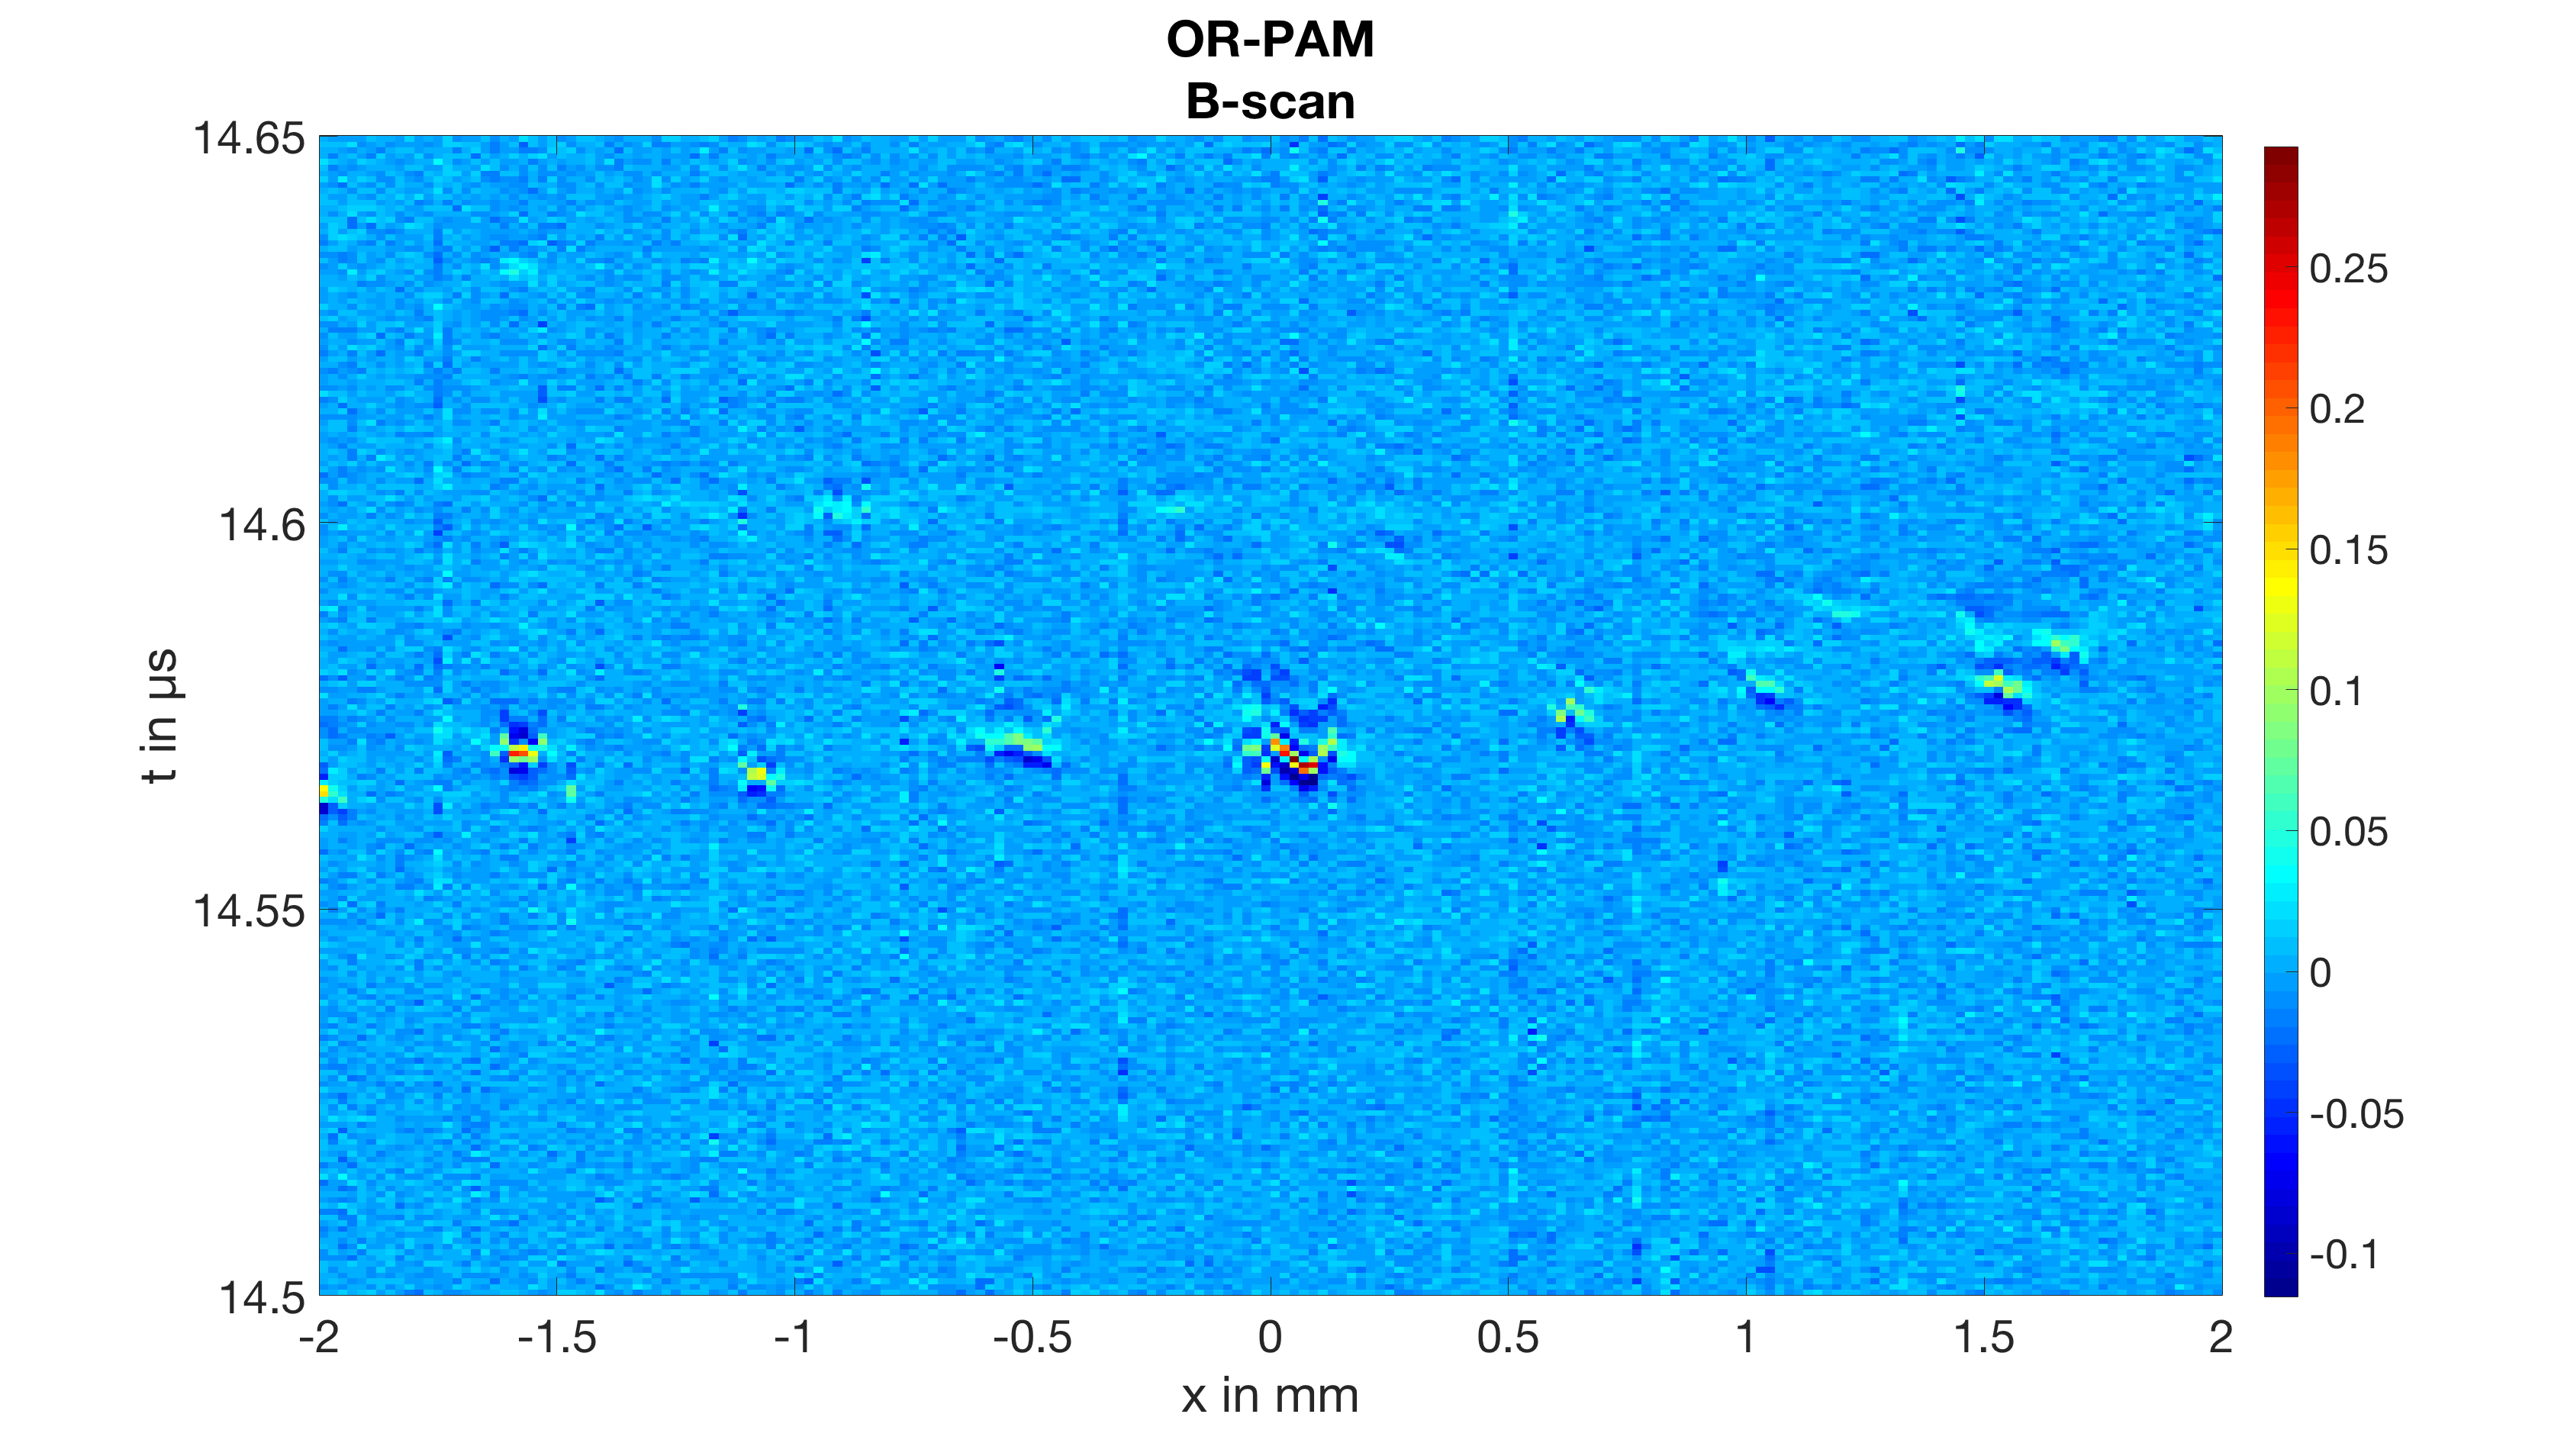
\includegraphics[width = \textwidth]{02_principles_of_photoacoustics/images/Bscan.png}
	\end{minipage}
	b)
	\begin{minipage}{\textwidth}		
		\centering
		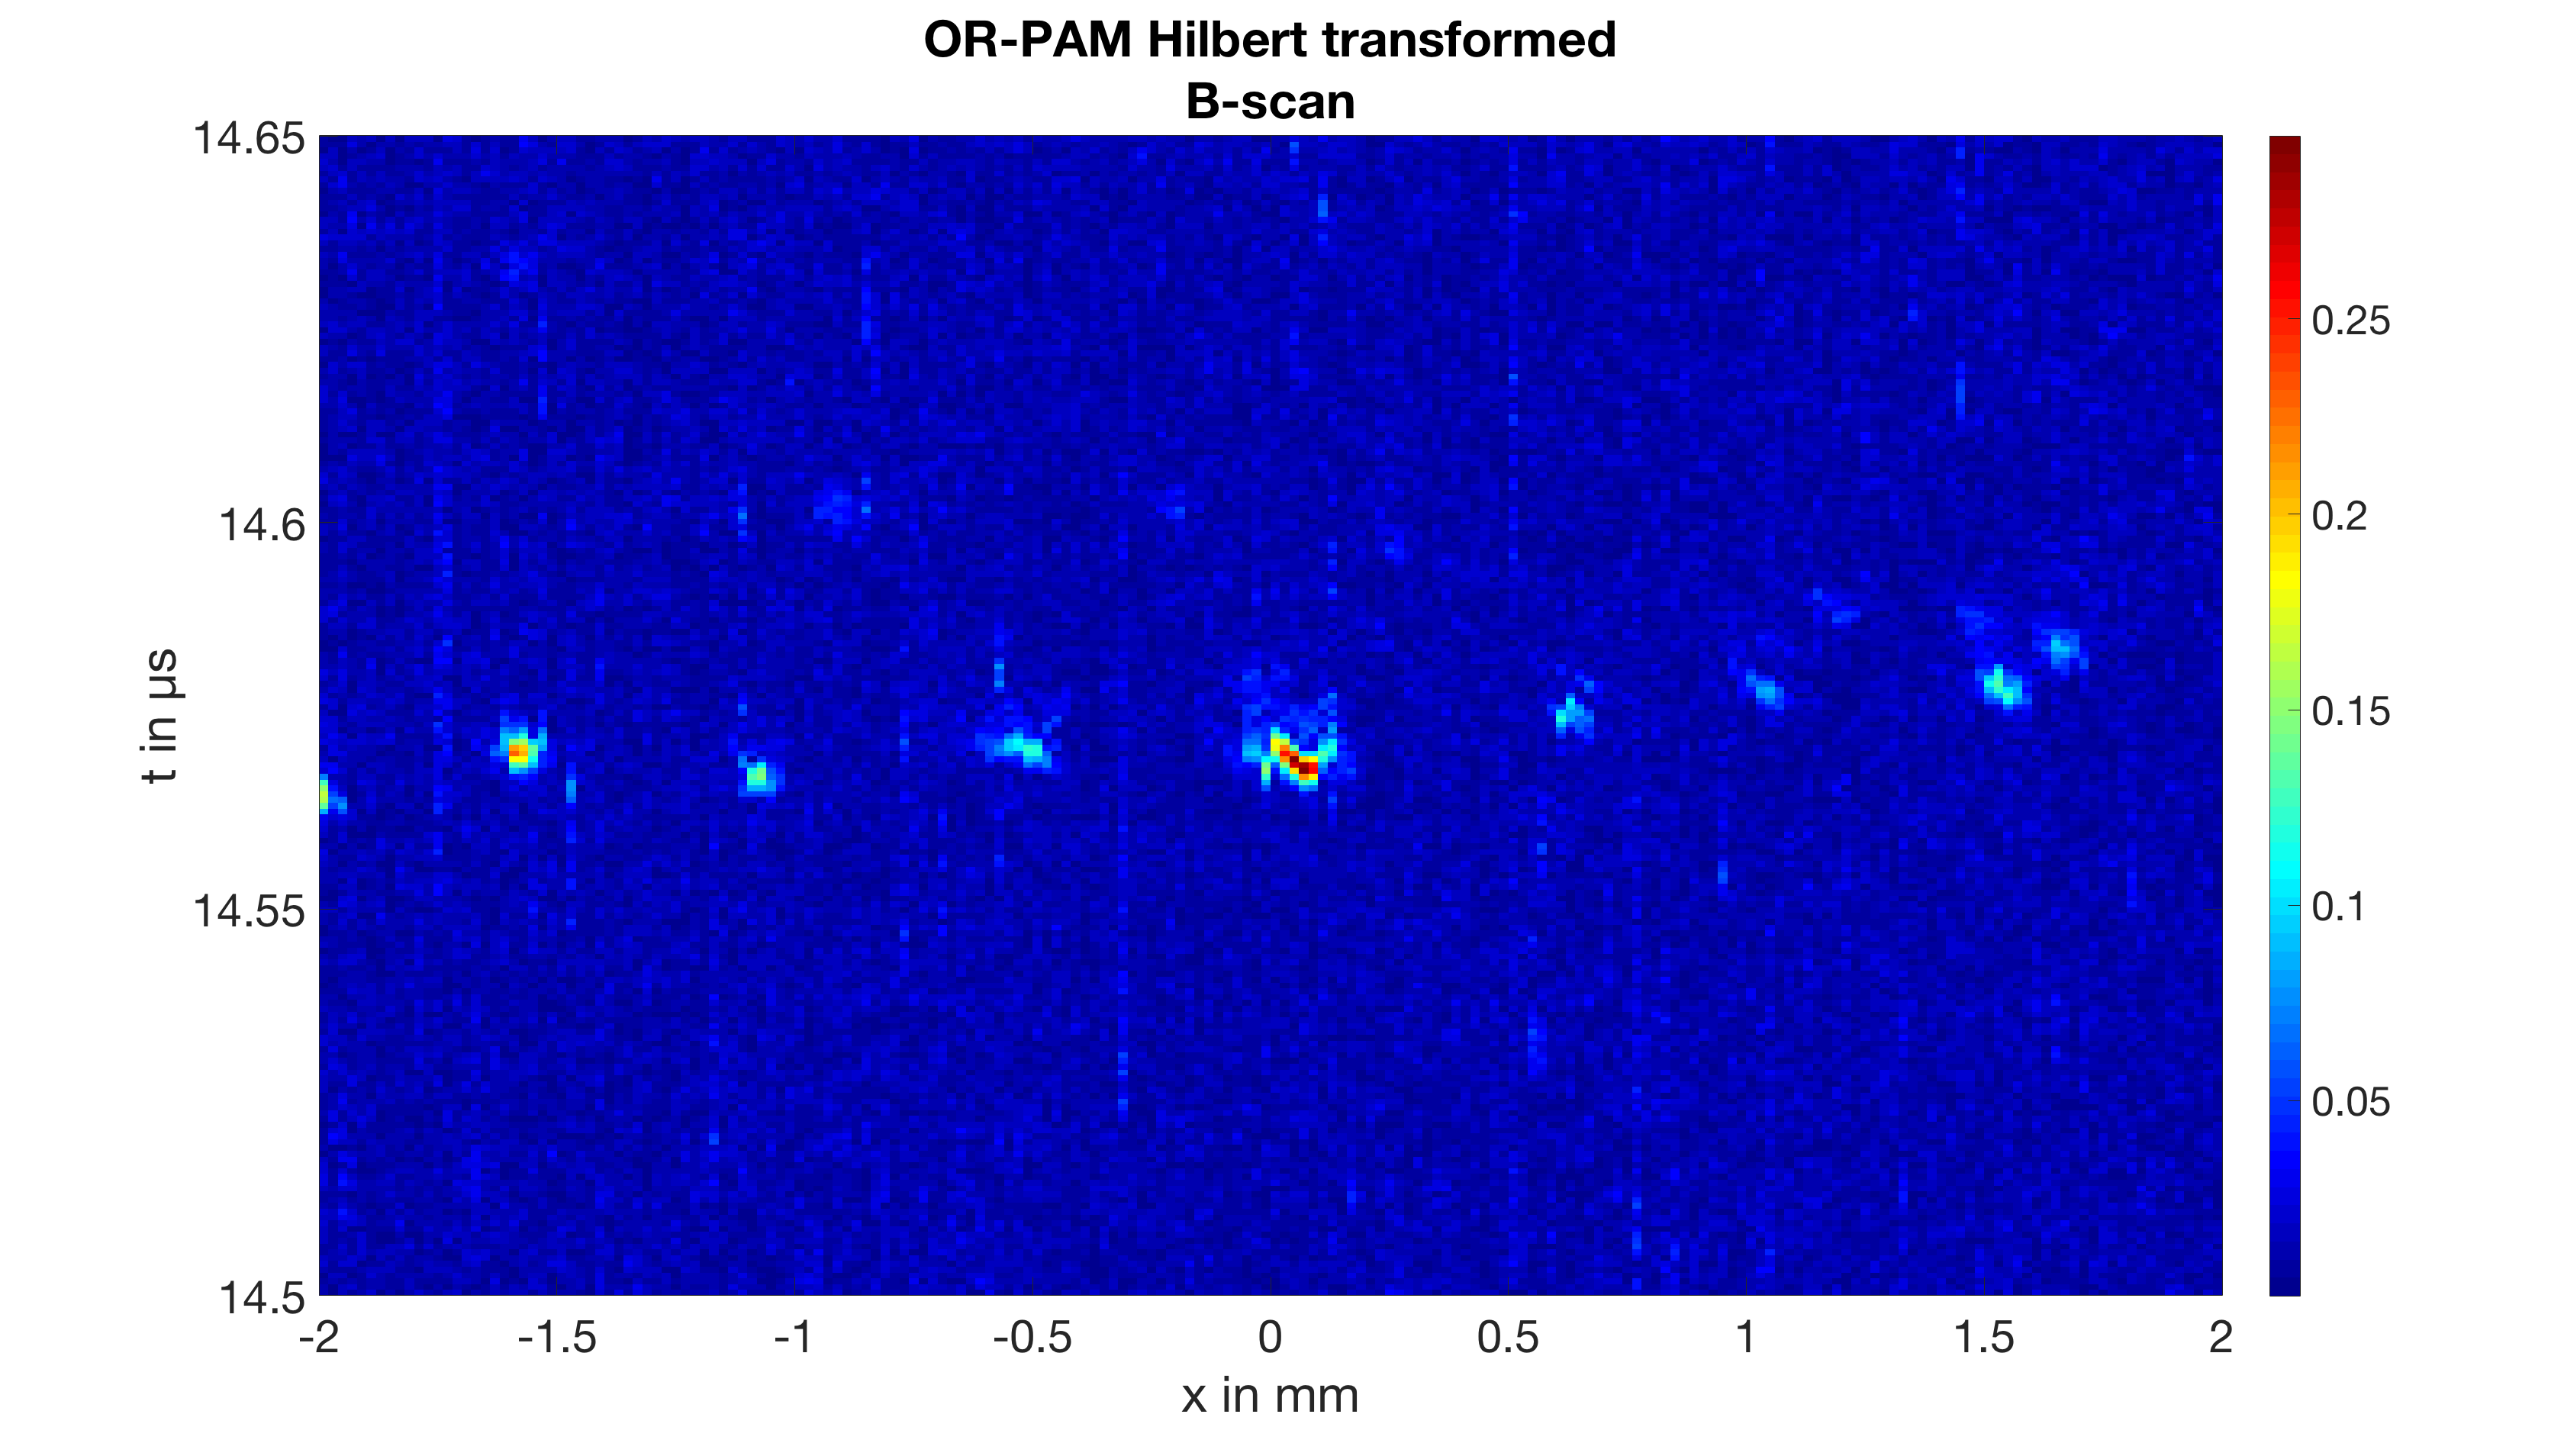
\includegraphics[width = \textwidth]{02_principles_of_photoacoustics/images/BscanHilbert.png}
	\end{minipage}	
	\caption{In a) a normal B-scan is shown and in b) its absolute value of the Hilbert transformed.}
	\label{fig:BsacanHilbert}
\end{figure}

In b) the effect is clearly visible, the SNR is observable higher than in a). \\
Therefore the HT is a efficient way to reduce noise in PAM images. 


